%!TEX root = thesis.tex

\begin{appendices}
\chapter{Categorical Information Boost Autoencoder Architecture Details} \label{ch:cibae-arch}
Similar to Segnet \citep{BadrinarayananK15}, our implementation uses a symmetric sequence of downsampling convolution modules (DownConvModule Fig.~\ref{fig:DownConvMod}) and upsampling convolution modules (UpConvModule Fig.~\ref{fig:UpConvMod}), where the spatial resolution changes by a factor of two at the end of each module. All convolutions are with kernel size 3, stride 1, and padding 1 so that the input and output spatial resolutions are identical.

\begin{lstlisting}[language=Python, caption=CIB-AE Architecture Detail, label=cibae_arch]]
CIB_AE(
    Encoder(
        DownConvModule(3, 64, 2),
        DownConvModule(64, 128, 3),
        DownConvModule(128, 256, 3),
        DownConvModule(256, 512, 3),
        DownConvModule(512, 512, 3),
        Reshape((4, 4, 512) -> (8192)),
        Dropout(p=0.25),
        Softmax()
    ), 
    Decoder(
        Reshape((8192) -> (4, 4, 512)),
        UpConvModule(512, 512, 3),
        UpConvModule(512, 256, 3)
        UpConvModule(256, 128, 3),
        UpConvModule(128, 64, 2),
        UpConvModule(64, 3, 2)
    )
)
\end{lstlisting}

In our experiments we found that the single Dropout layer before the Softmax in the encoder was crucial. Without dropout, the encodings become overly sensitive to differences in the input images, and approximate encodings through our topic model and topic mapping algorithms are too different from real encodings to produce reasonable predictions.

\begin{figure}
    \begin{center}
    \subfloat[]{
        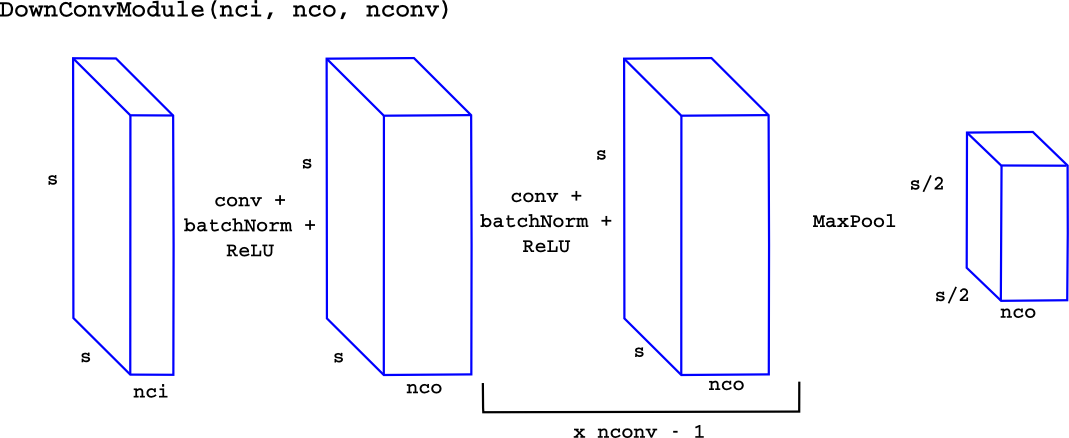
\includegraphics[width=0.9\columnwidth]{figures/ptz/DownConvModule.png}
        \label{fig:DownConvMod}
    }\\
    \subfloat[]{
        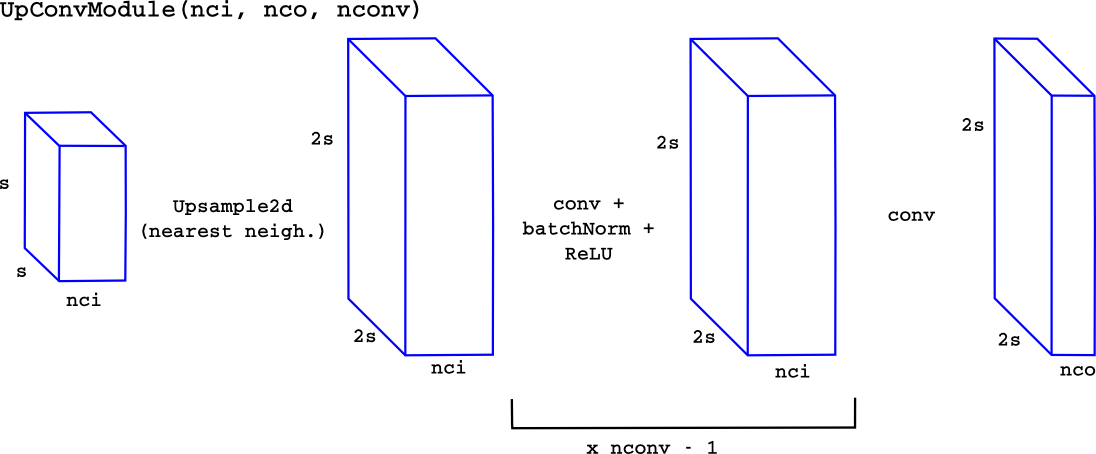
\includegraphics[width=0.9\columnwidth]{figures/ptz/UpConvModule.png}
        \label{fig:UpConvMod}
    }
    \end{center}
    \caption{
    \protect\subref{fig:DownConvMod} DownConv and \protect\subref{fig:UpConvMod} UpConv modules used in our architecture. nci stands for number of channels in, nco number of channels out, and s the spatial resolution of the input representation. In our model, $nco = 2 nci$ for DownConvModules and $nco = nci/2$ for UpConvModules. Each block is made of a sequence of convolution, batch norm, and nonlinear activation blocks. The last convolution of the UpConvModule does not include the batch norm and nonlinearities because the training images are standardized (i.e. pixel values can be both negative and positive).
    }
    \label{fig:cib-ae_modules}
\end{figure}

\chapter{Supplemental View Predictions} \label{ch:app-predictions}
\section{Observed Views}
\begin{figure}[H]
    \centering
    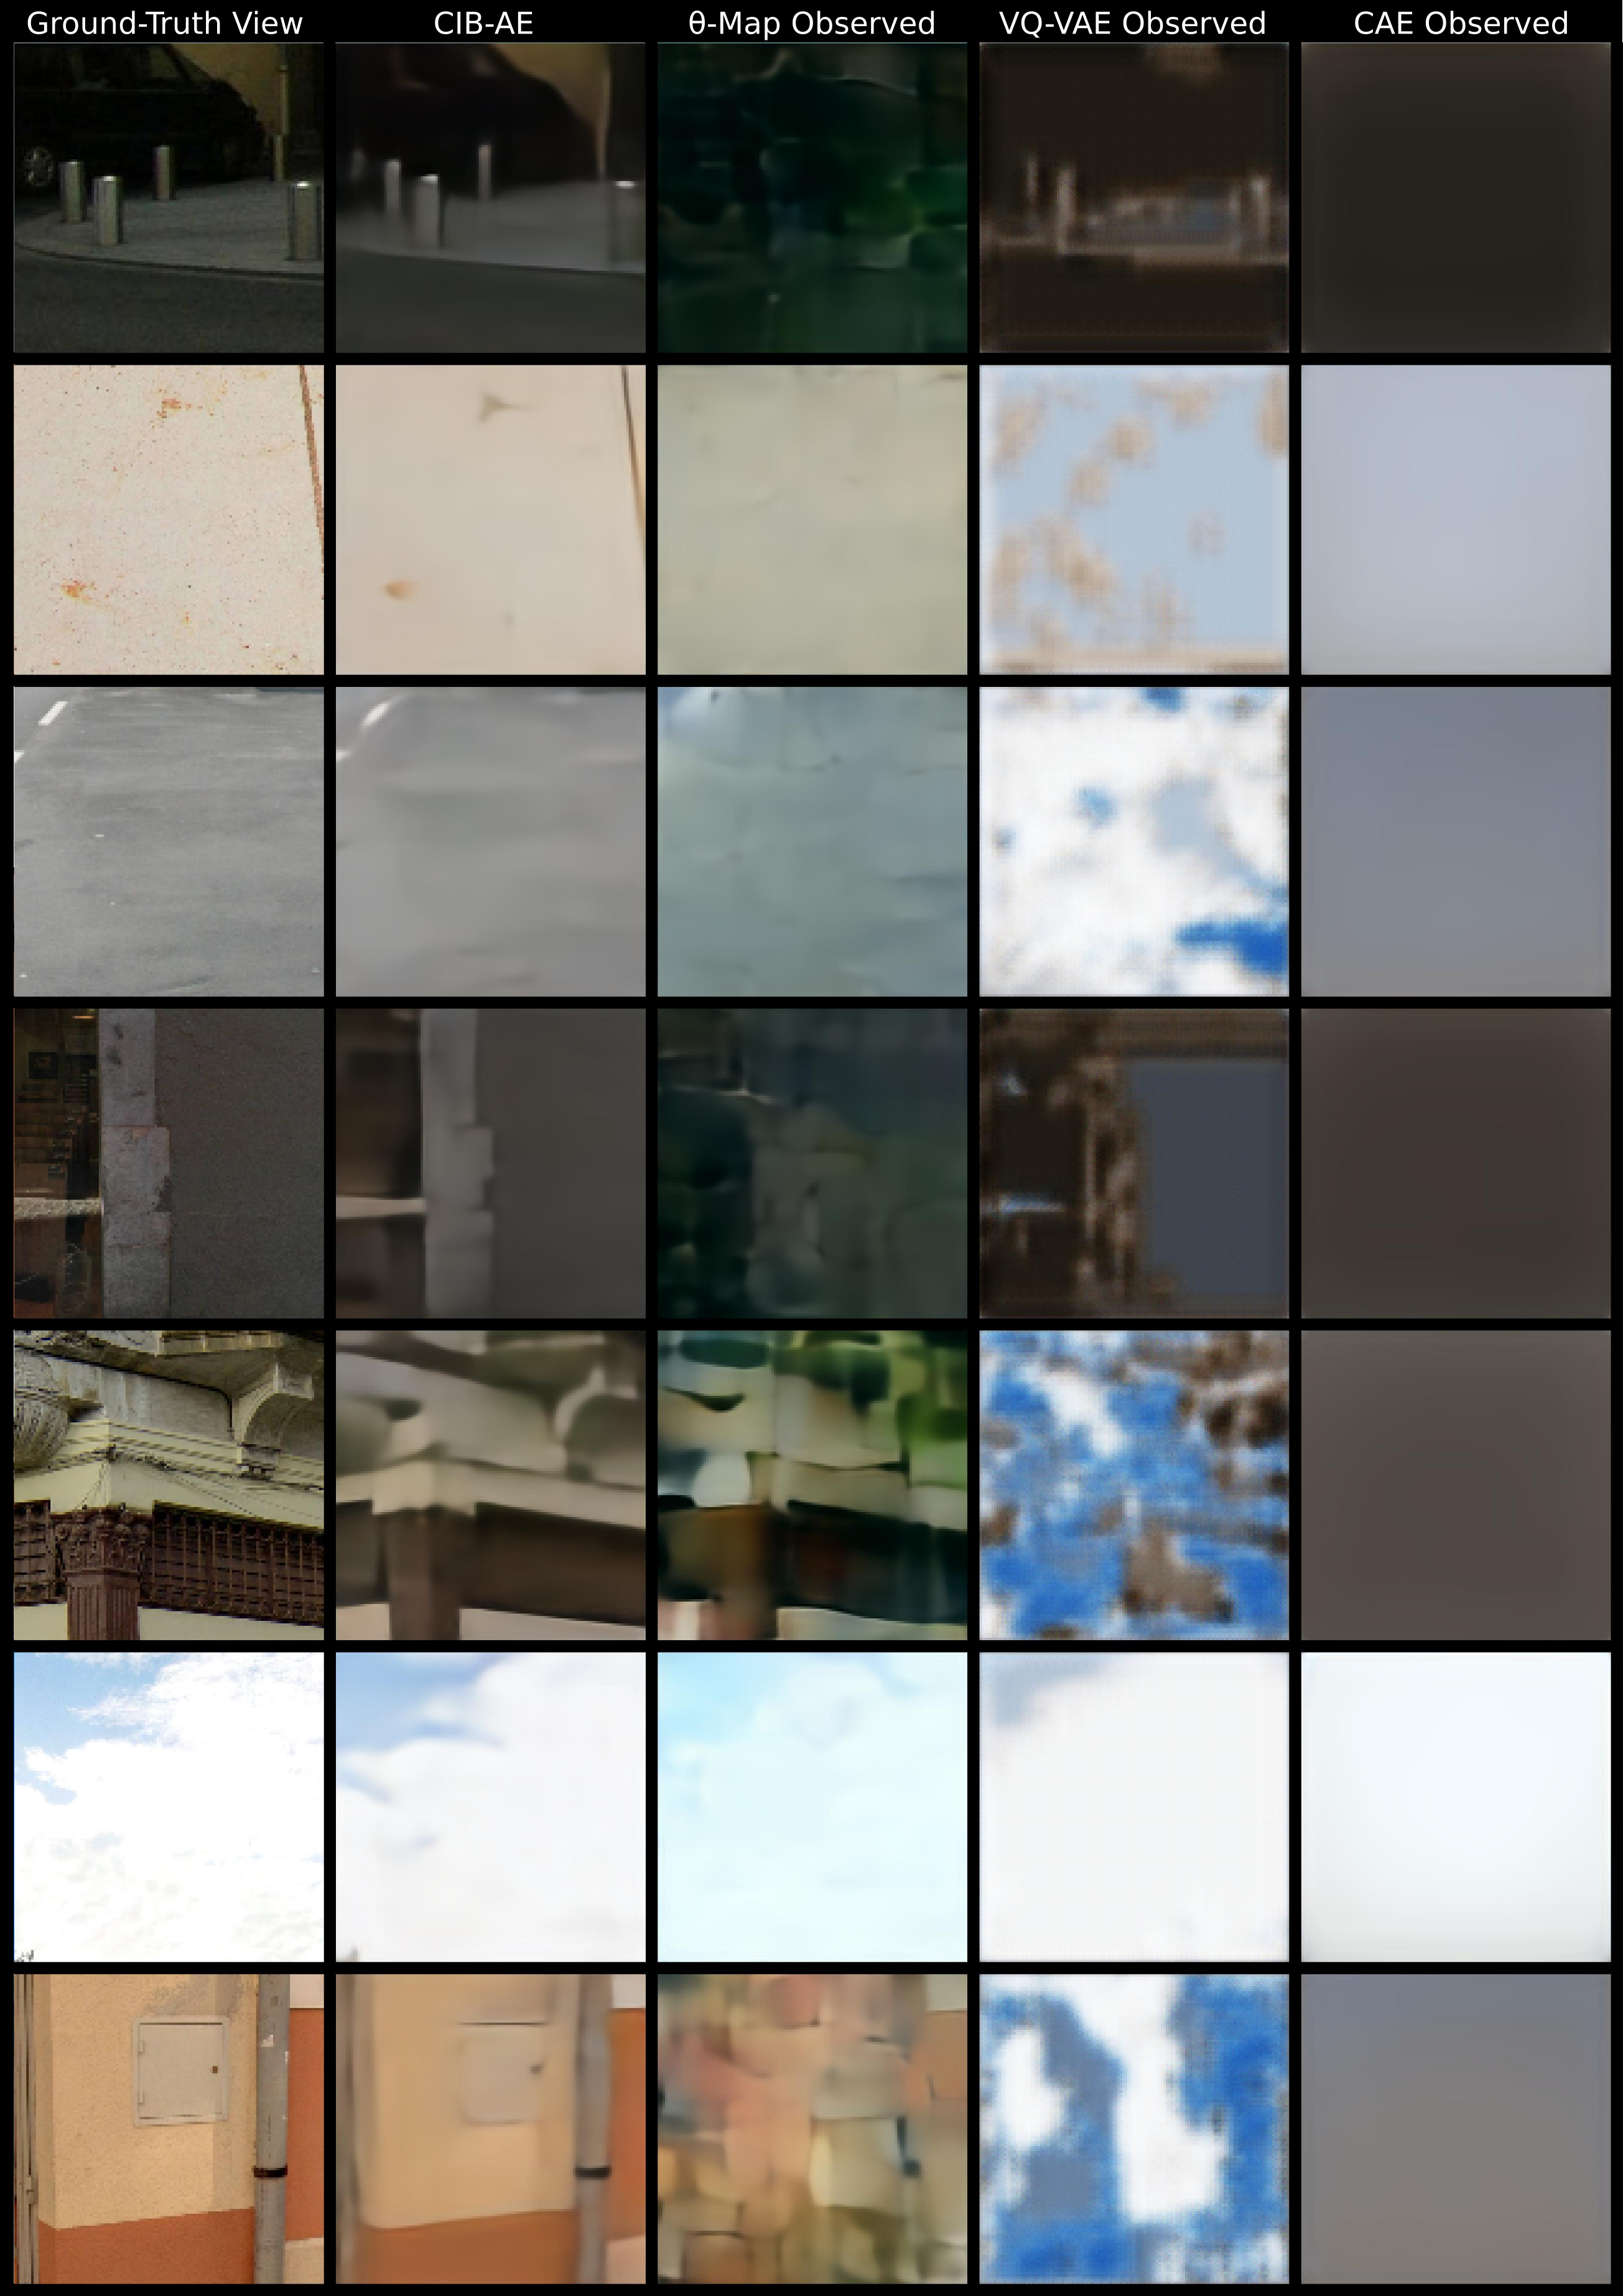
\includegraphics[width=0.85\textwidth]{figures/ptz/train_stacked_0.png}
\end{figure}
\begin{figure}[H]
    \centering
    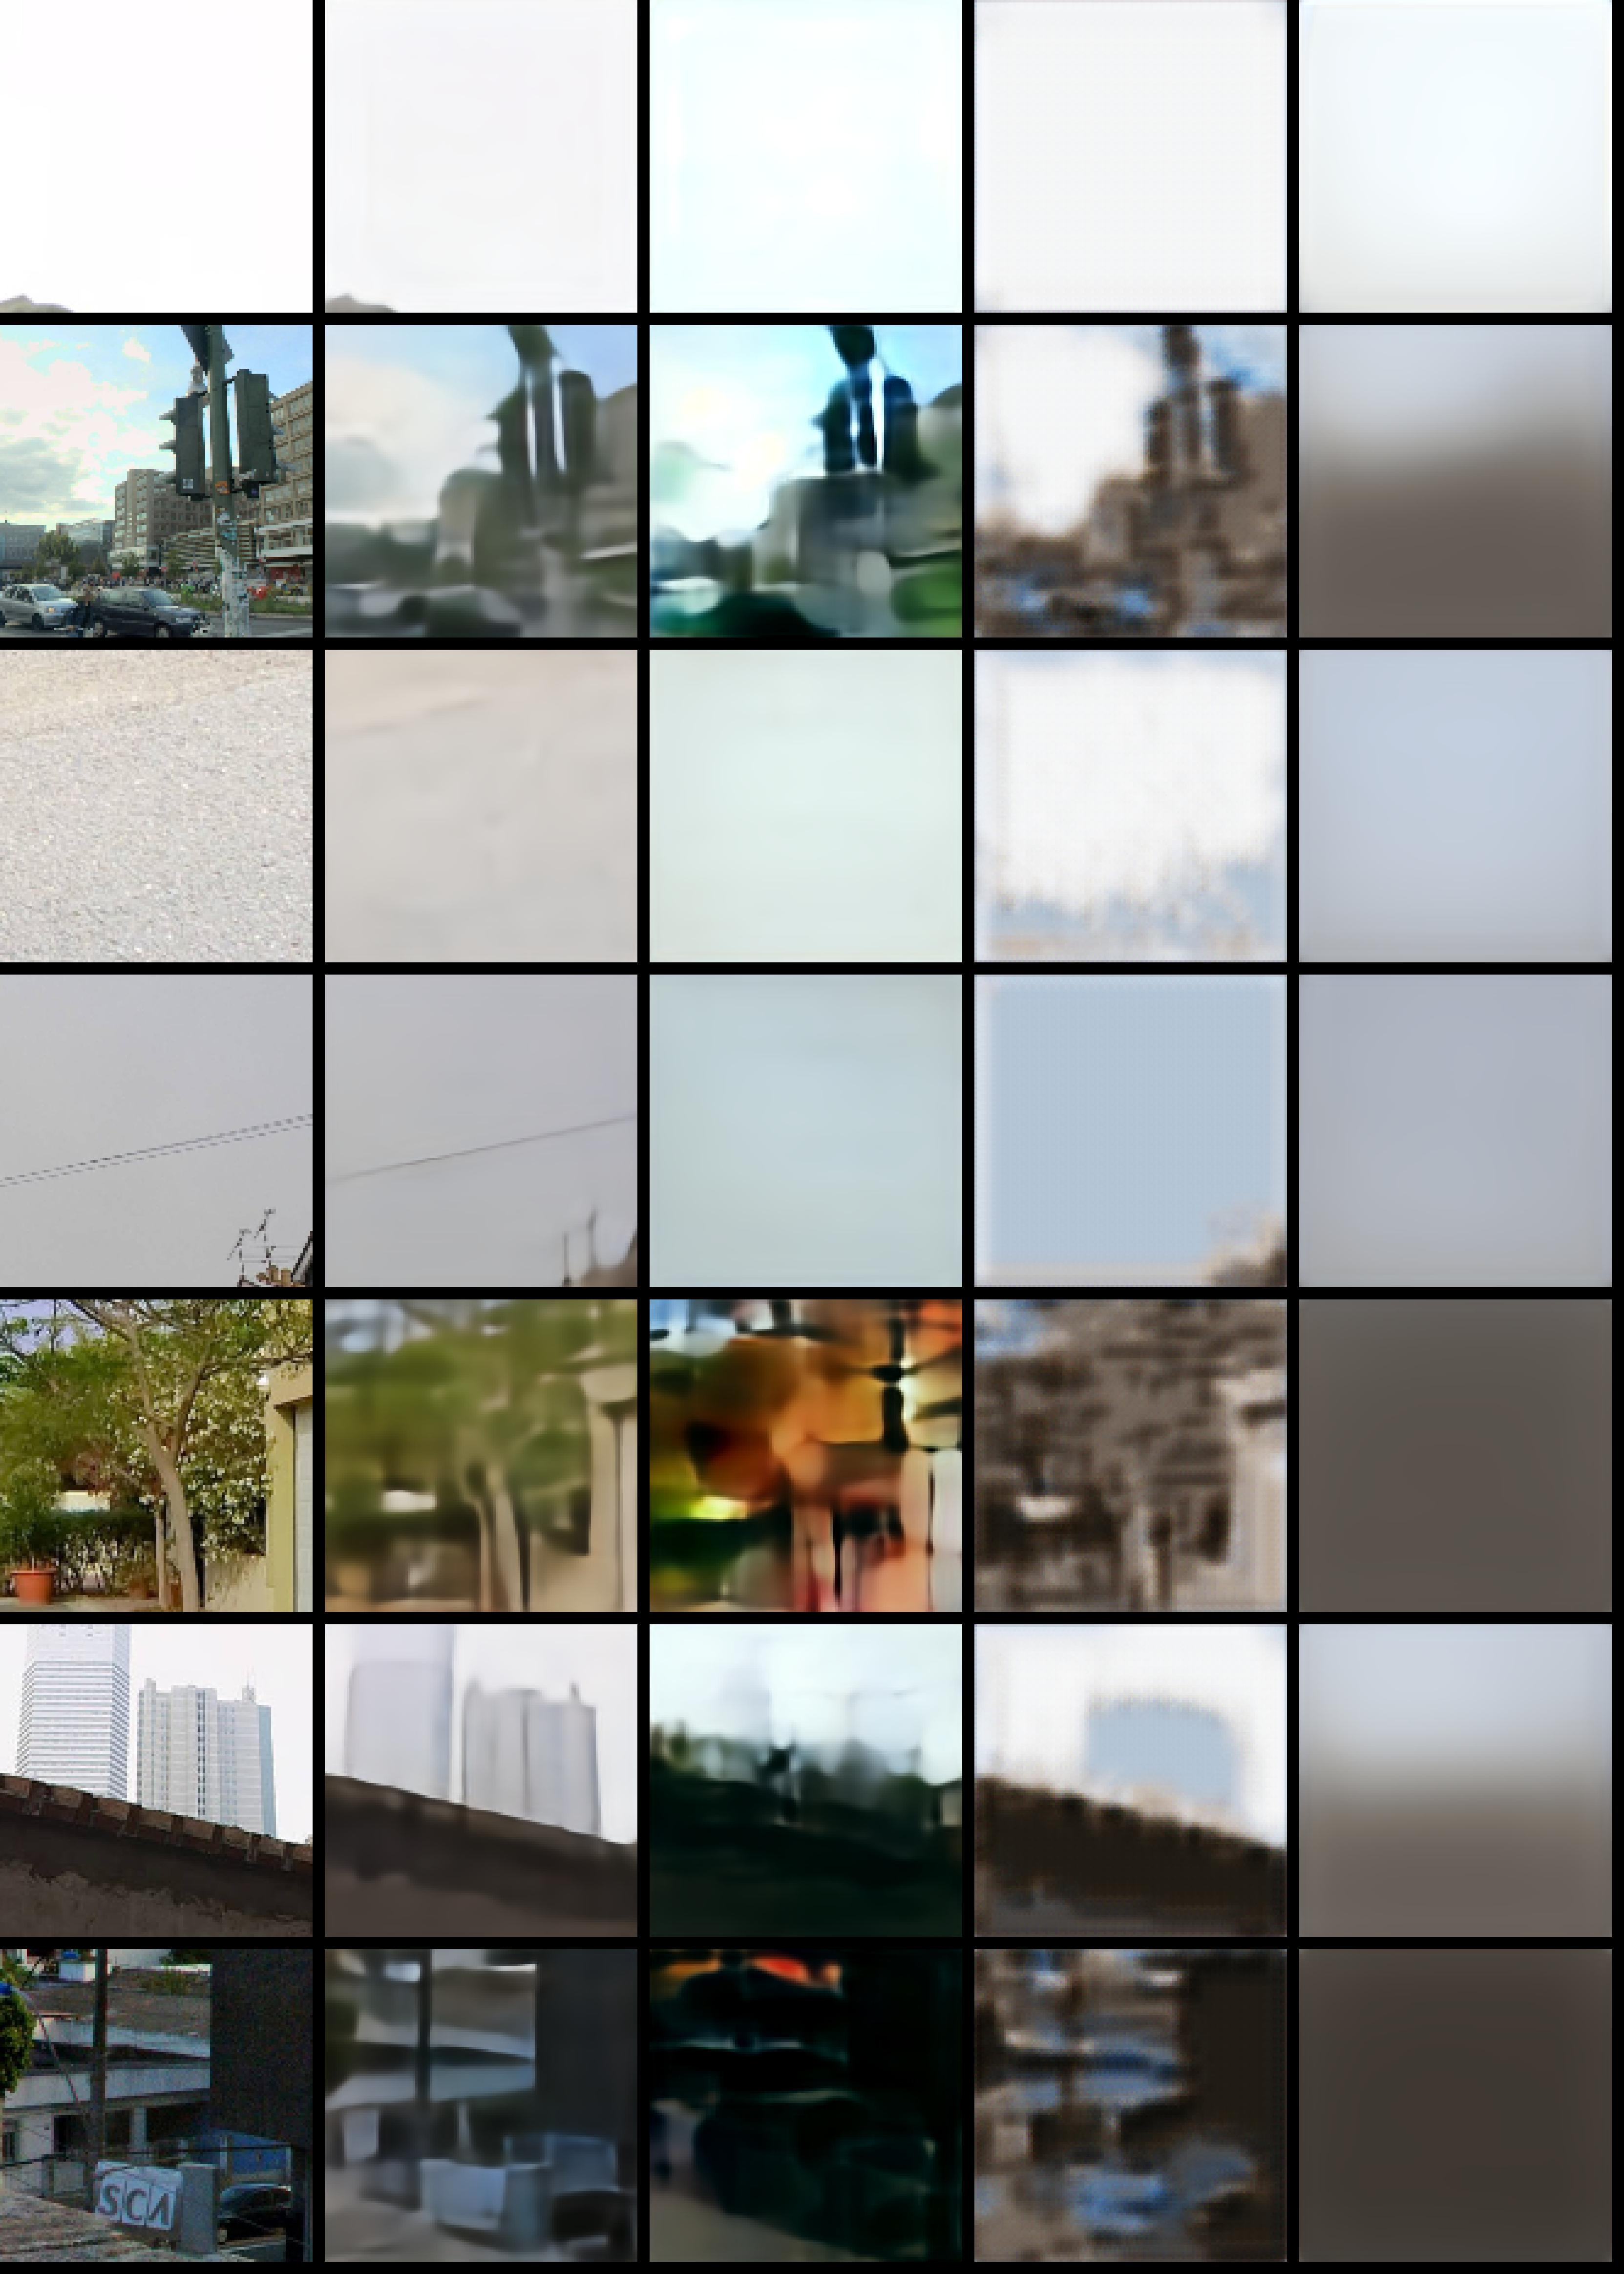
\includegraphics[width=0.85\textwidth]{figures/ptz/train_stacked_1.png}
\end{figure}
\begin{figure}[H]
    \centering
    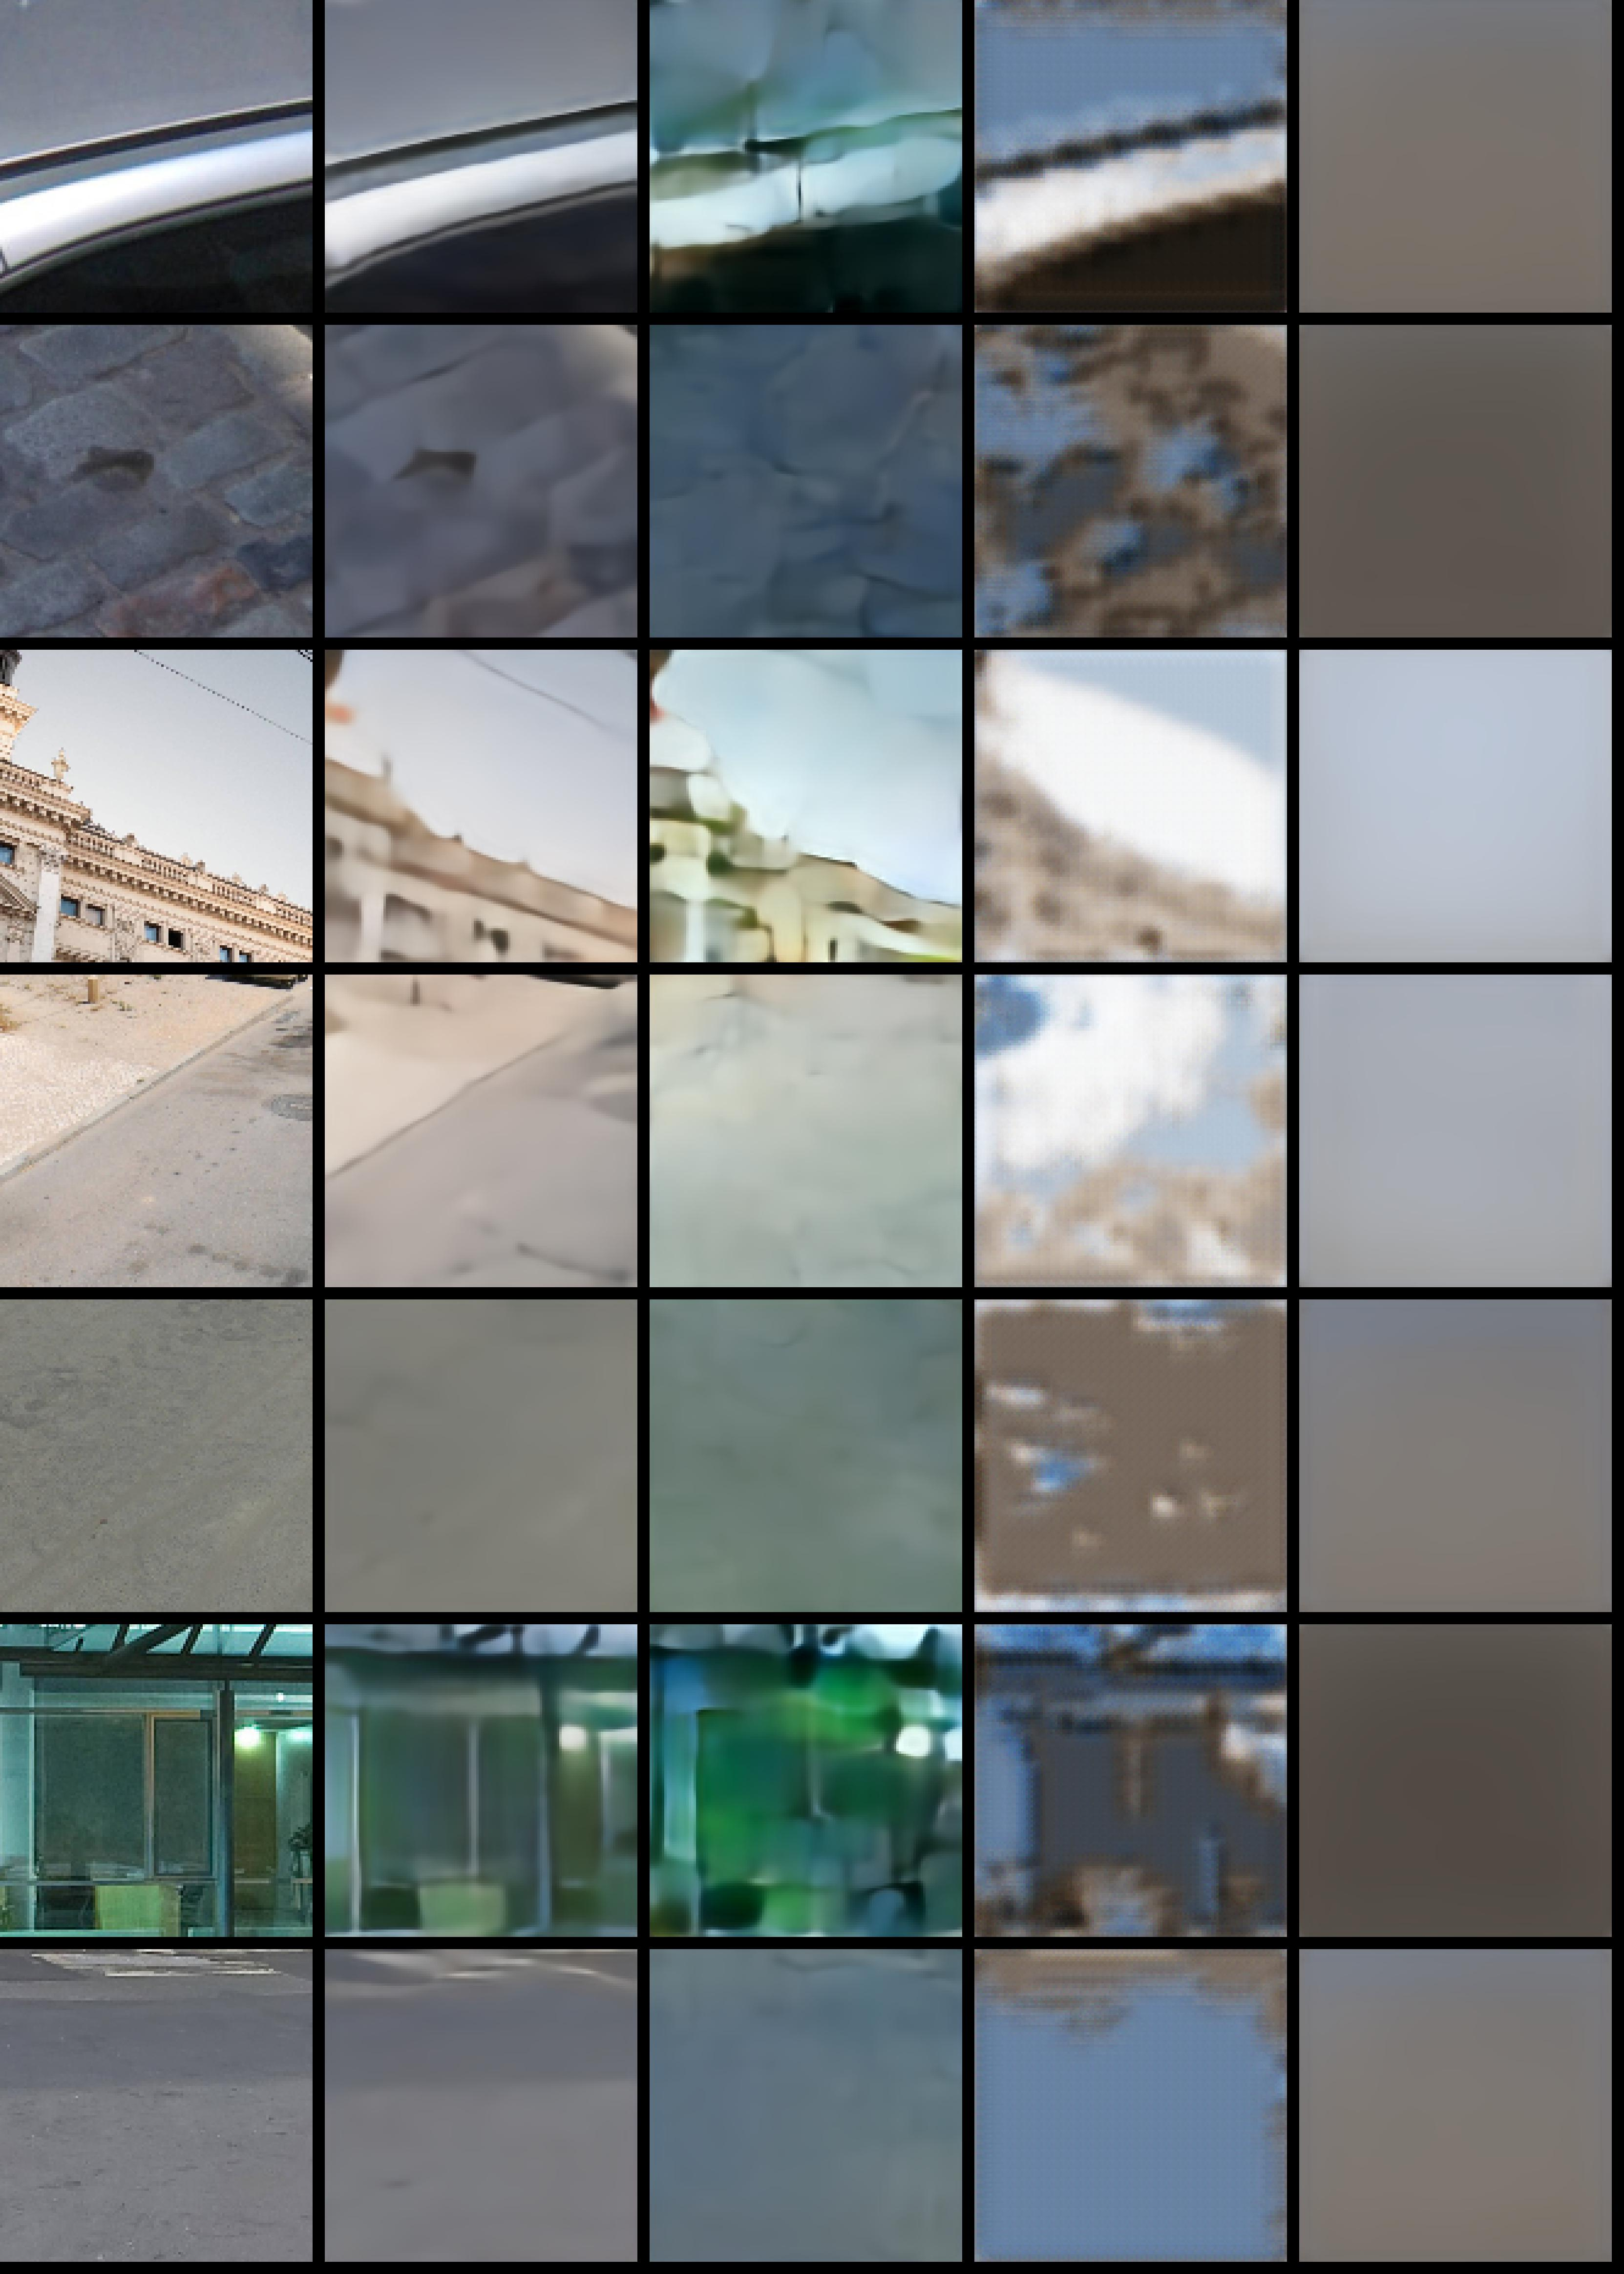
\includegraphics[width=0.85\textwidth]{figures/ptz/train_stacked_2.png}
\end{figure}
\begin{figure}[H]
    \centering
    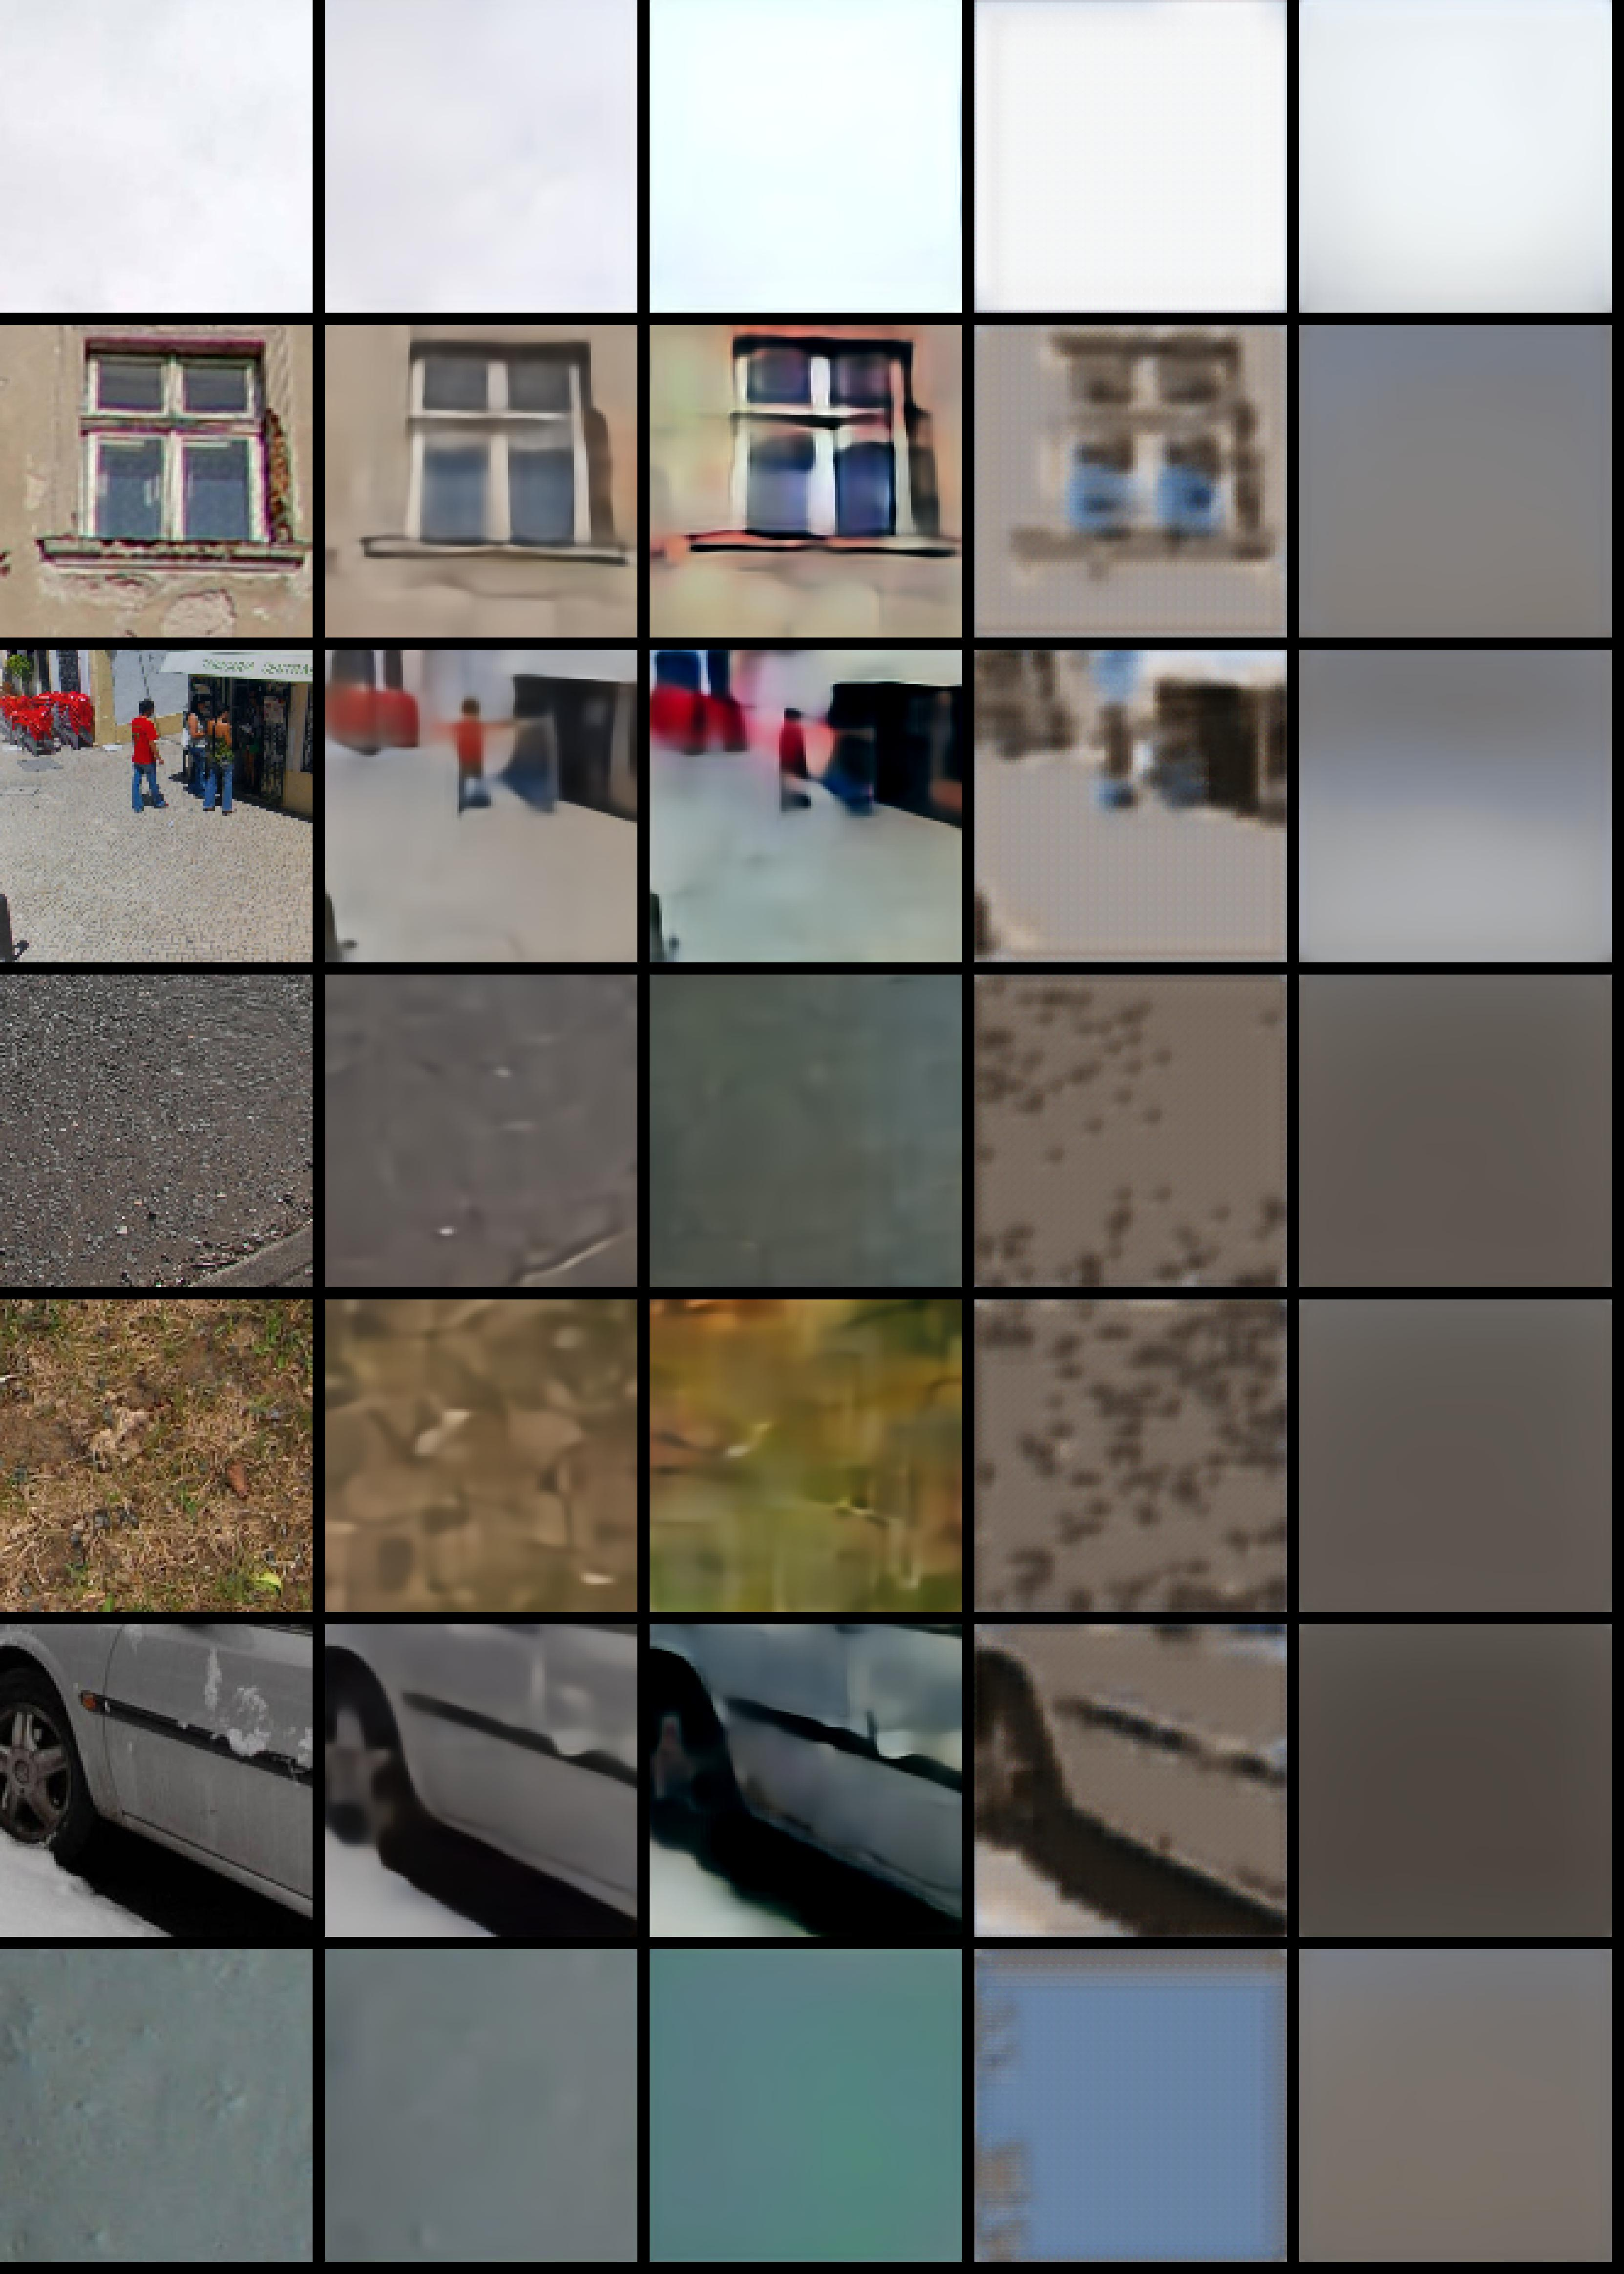
\includegraphics[width=0.85\textwidth]{figures/ptz/train_stacked_3.png}
\end{figure}
\begin{figure}[H]
    \centering
    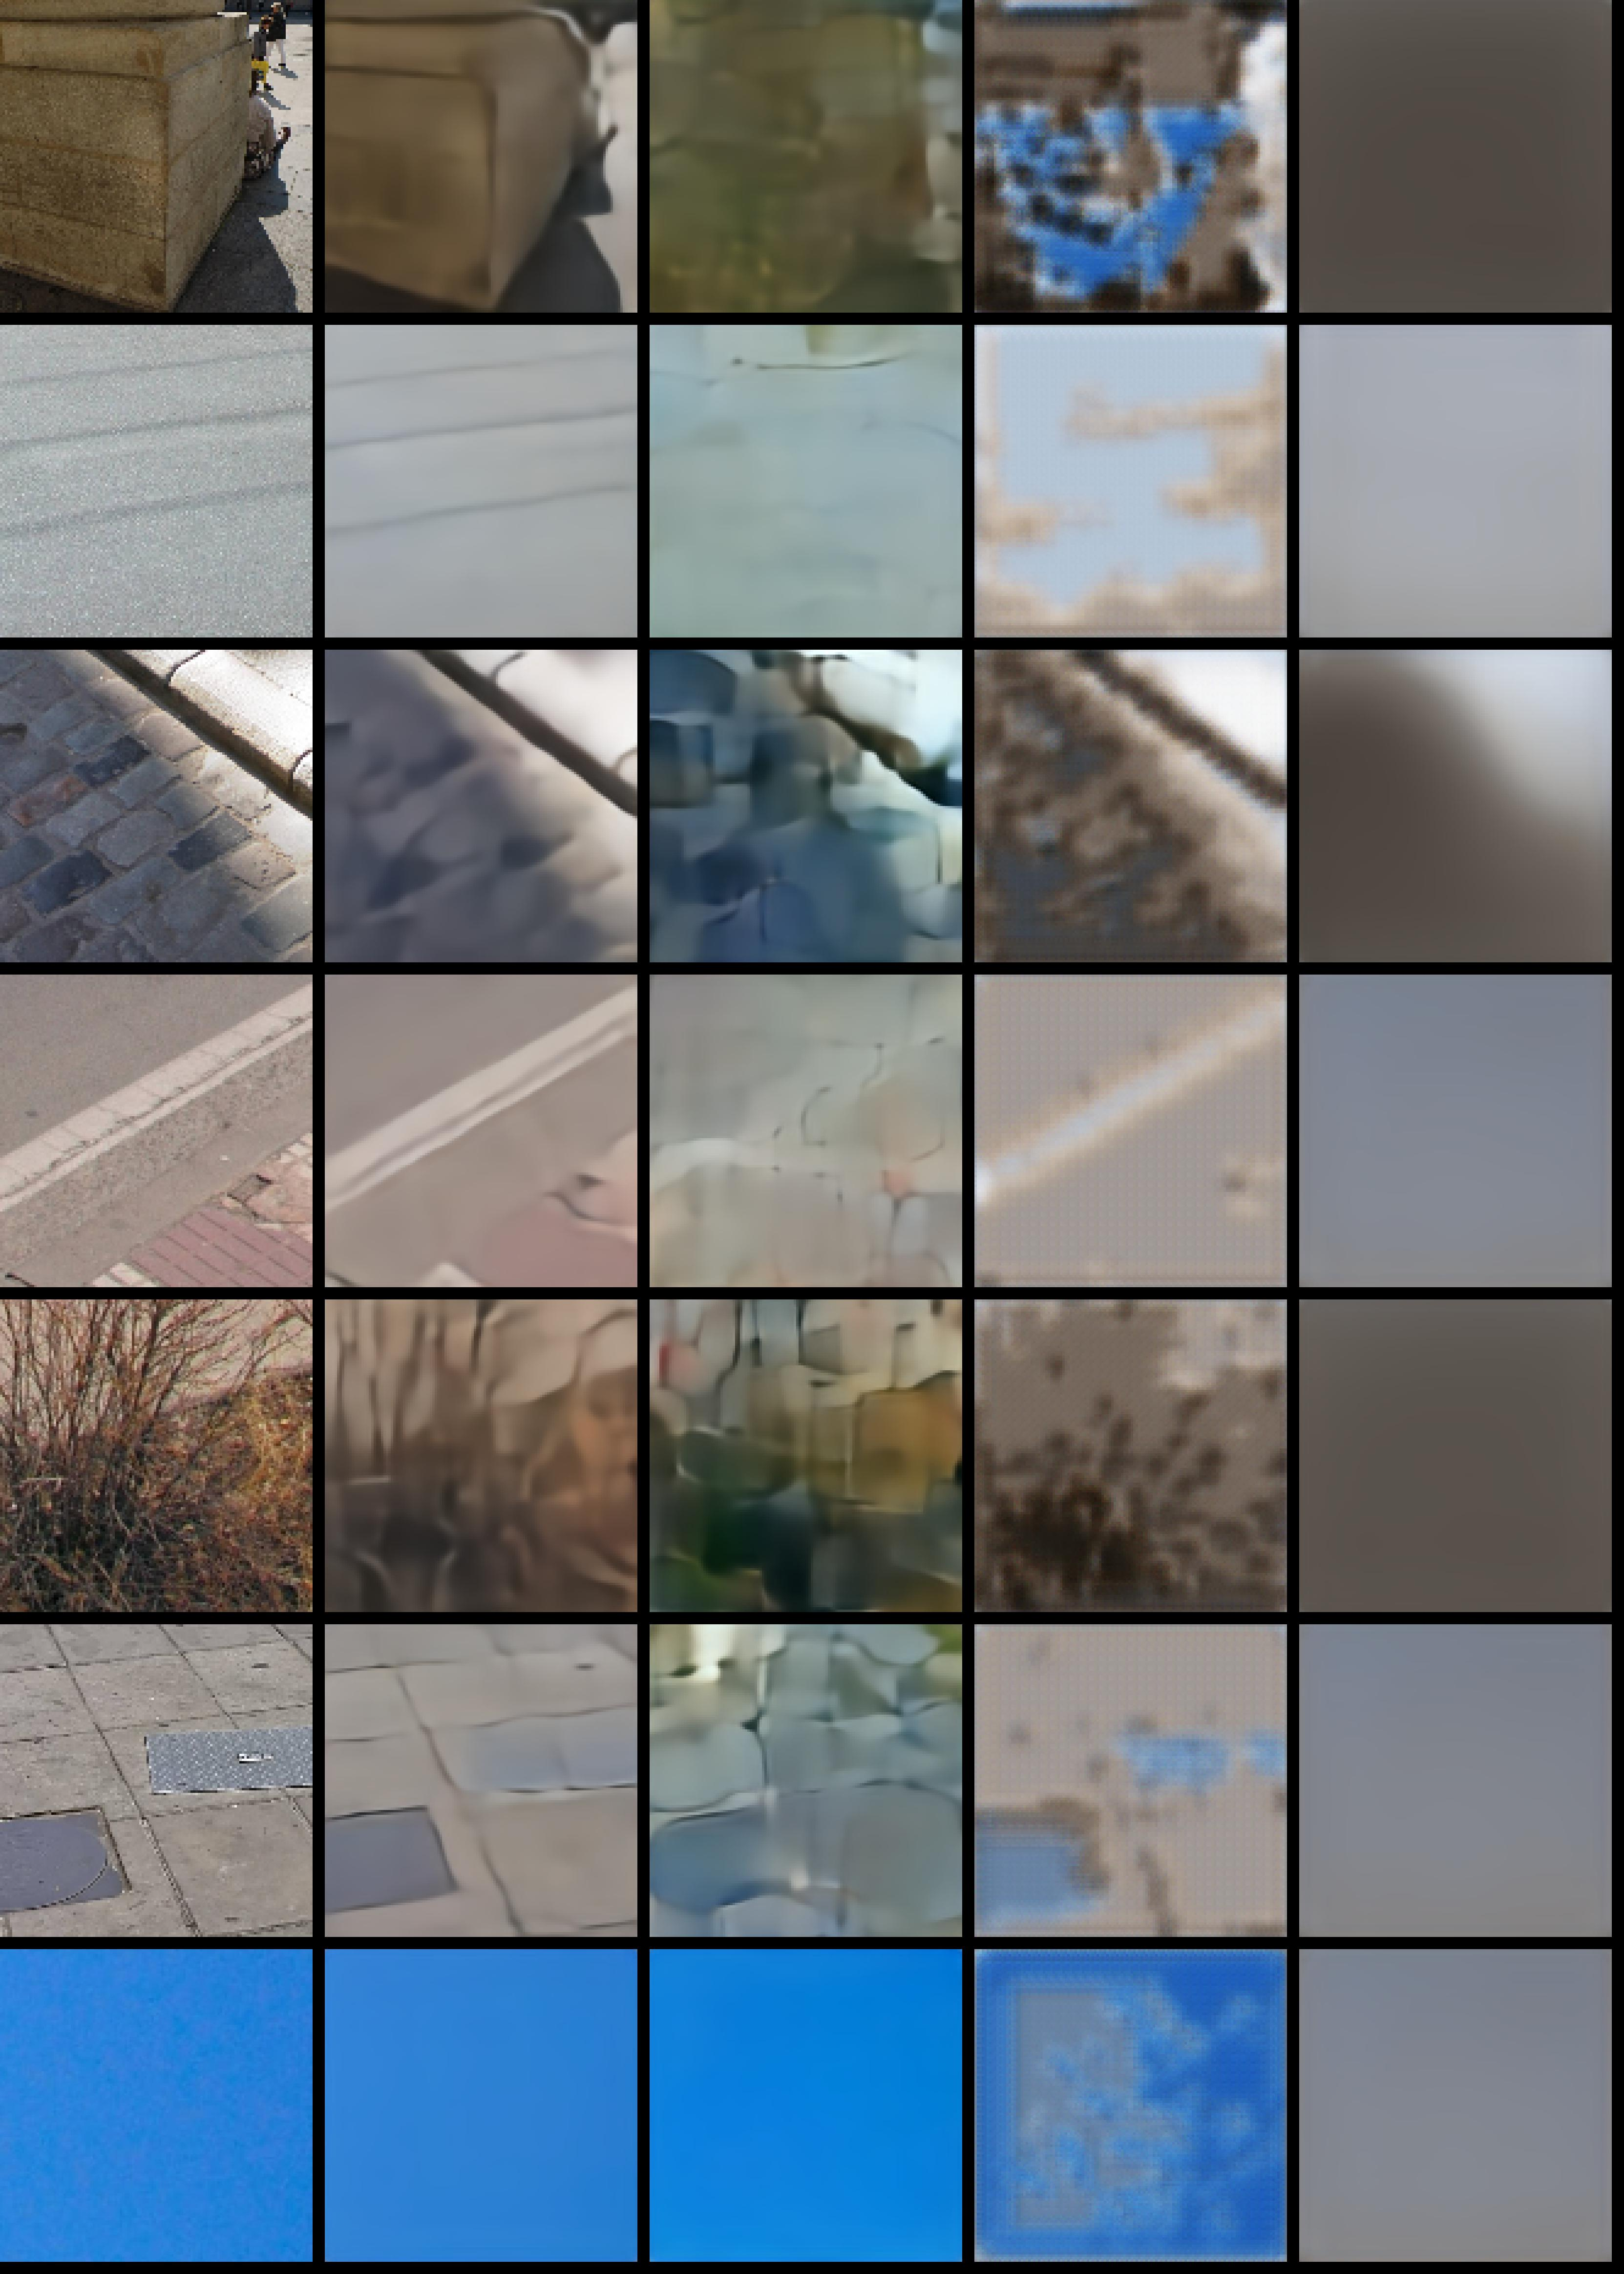
\includegraphics[width=0.85\textwidth]{figures/ptz/train_stacked_4.png}
\end{figure}

\section{Predicted Views}
\begin{figure}[H]
    \centering
    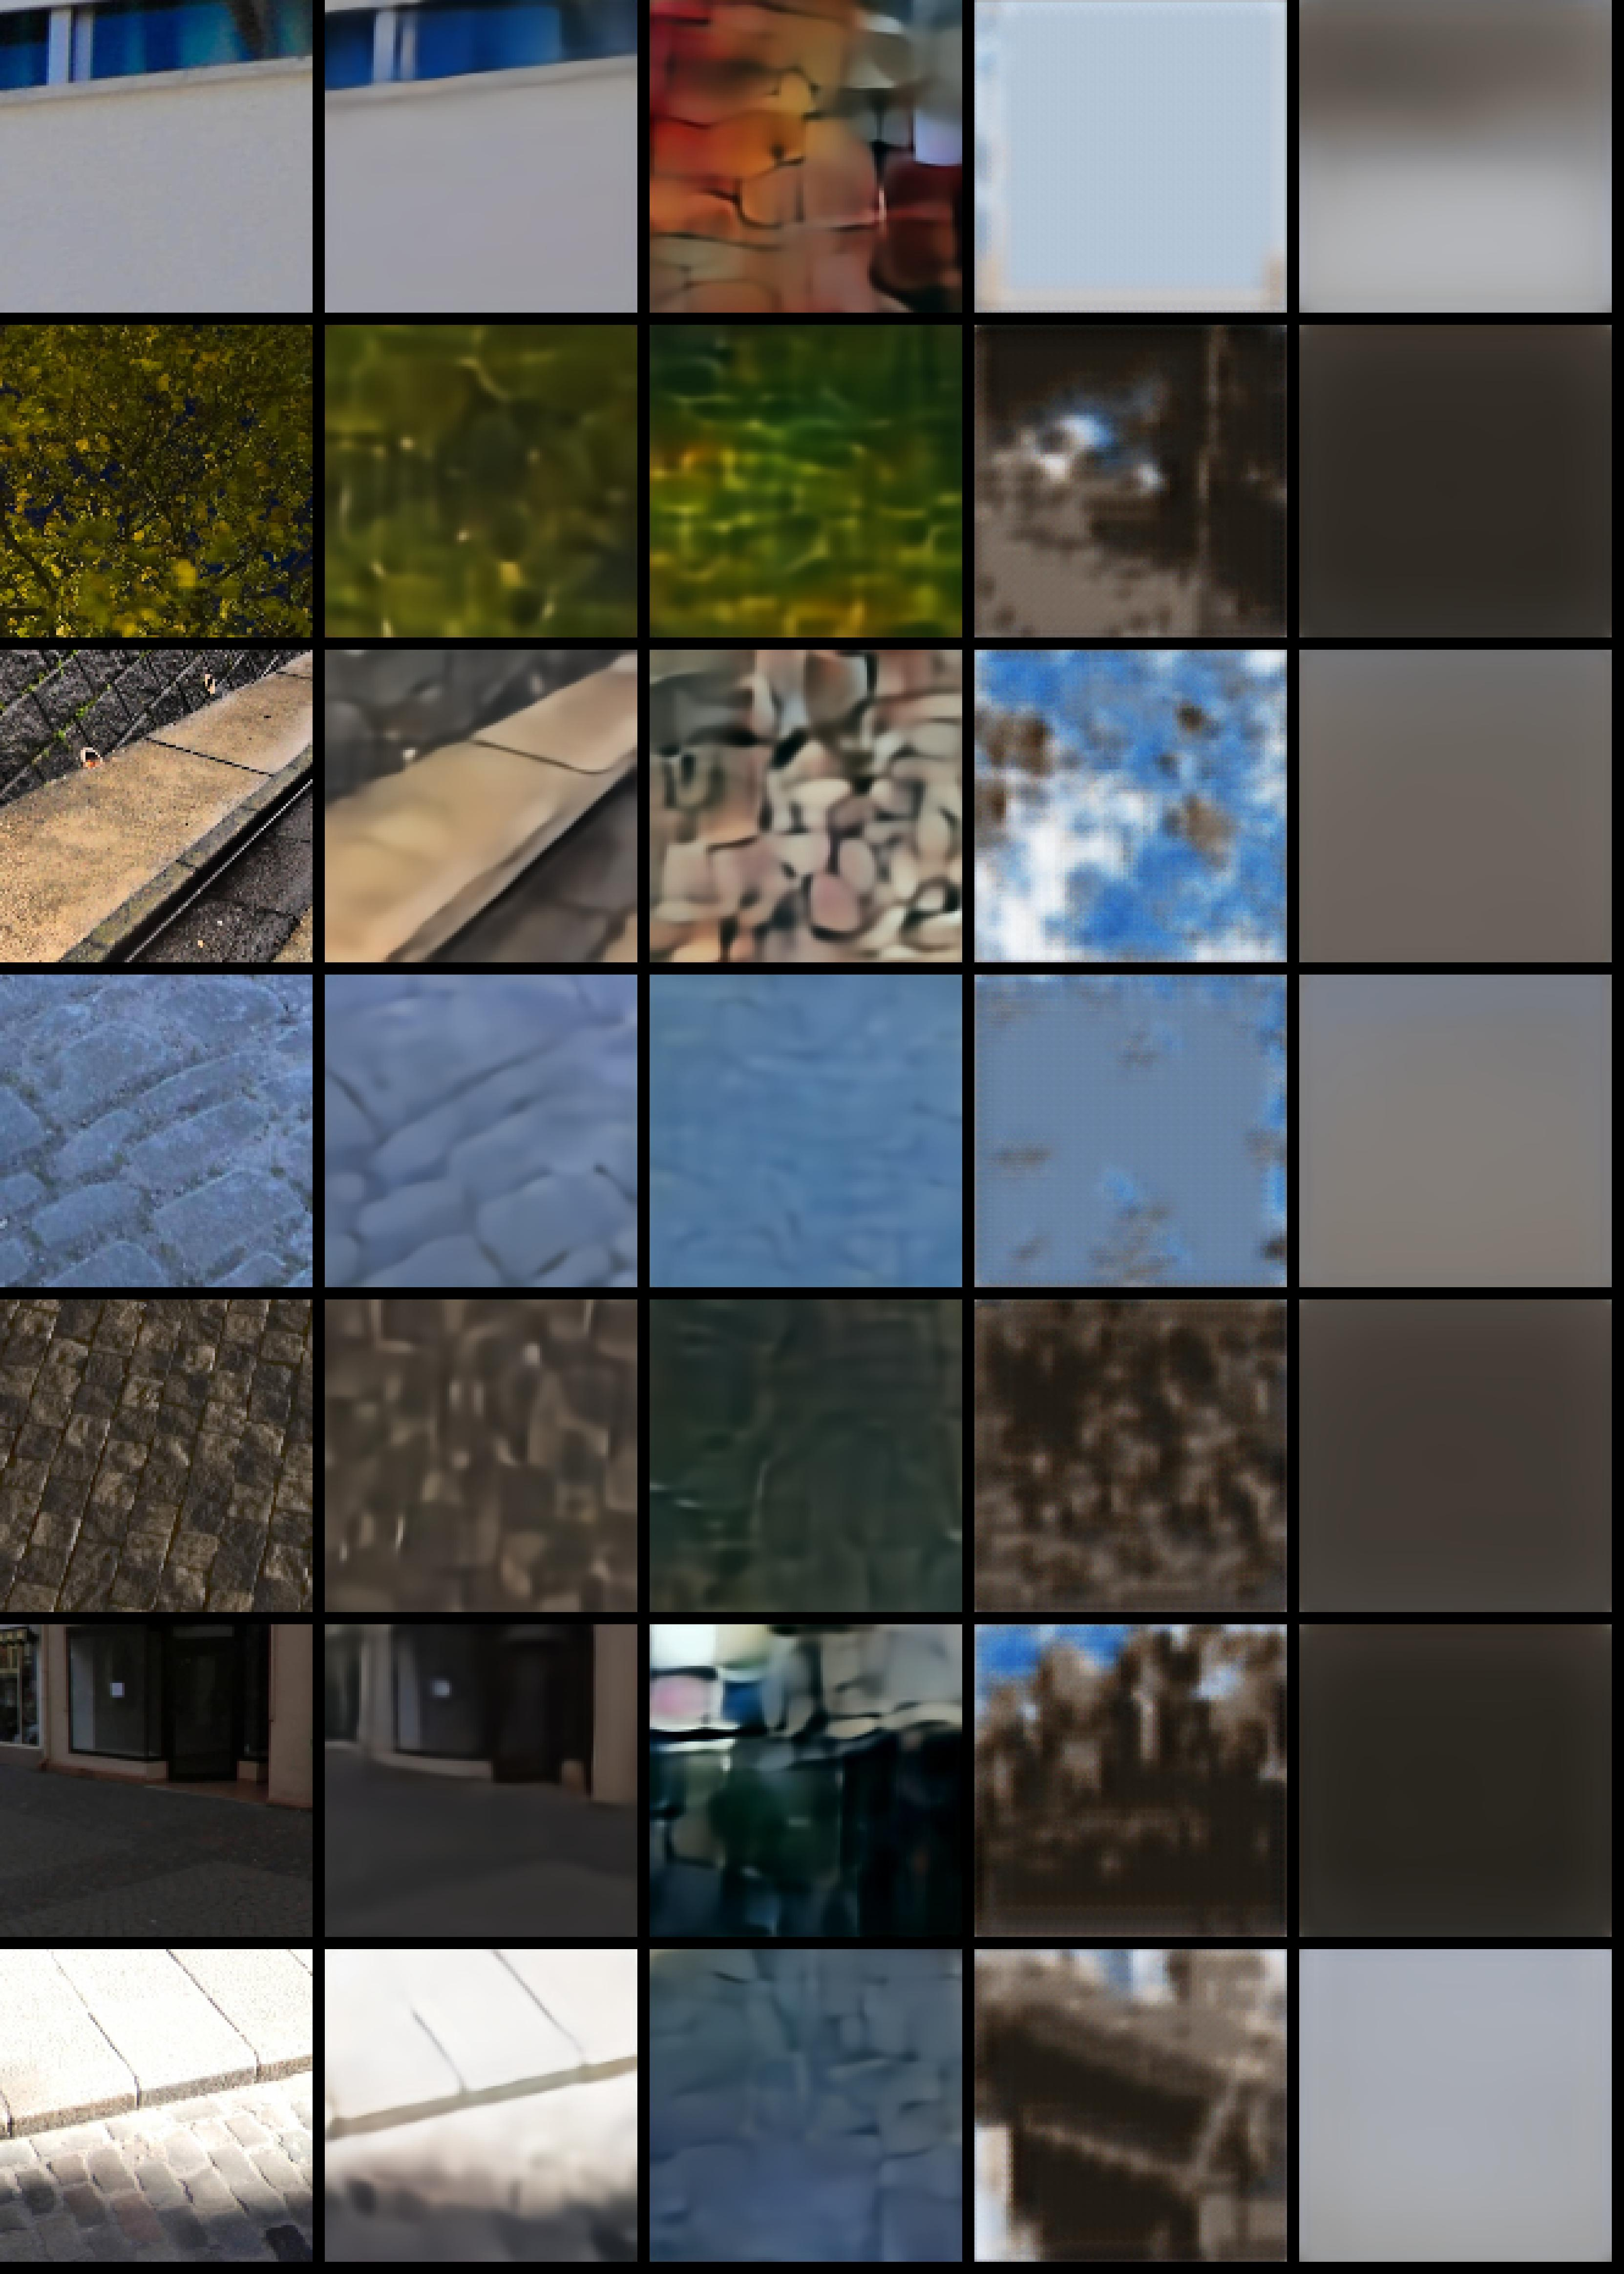
\includegraphics[width=0.85\textwidth]{figures/ptz/test_stacked_0.png}
\end{figure}
\begin{figure}[H]
    \centering
    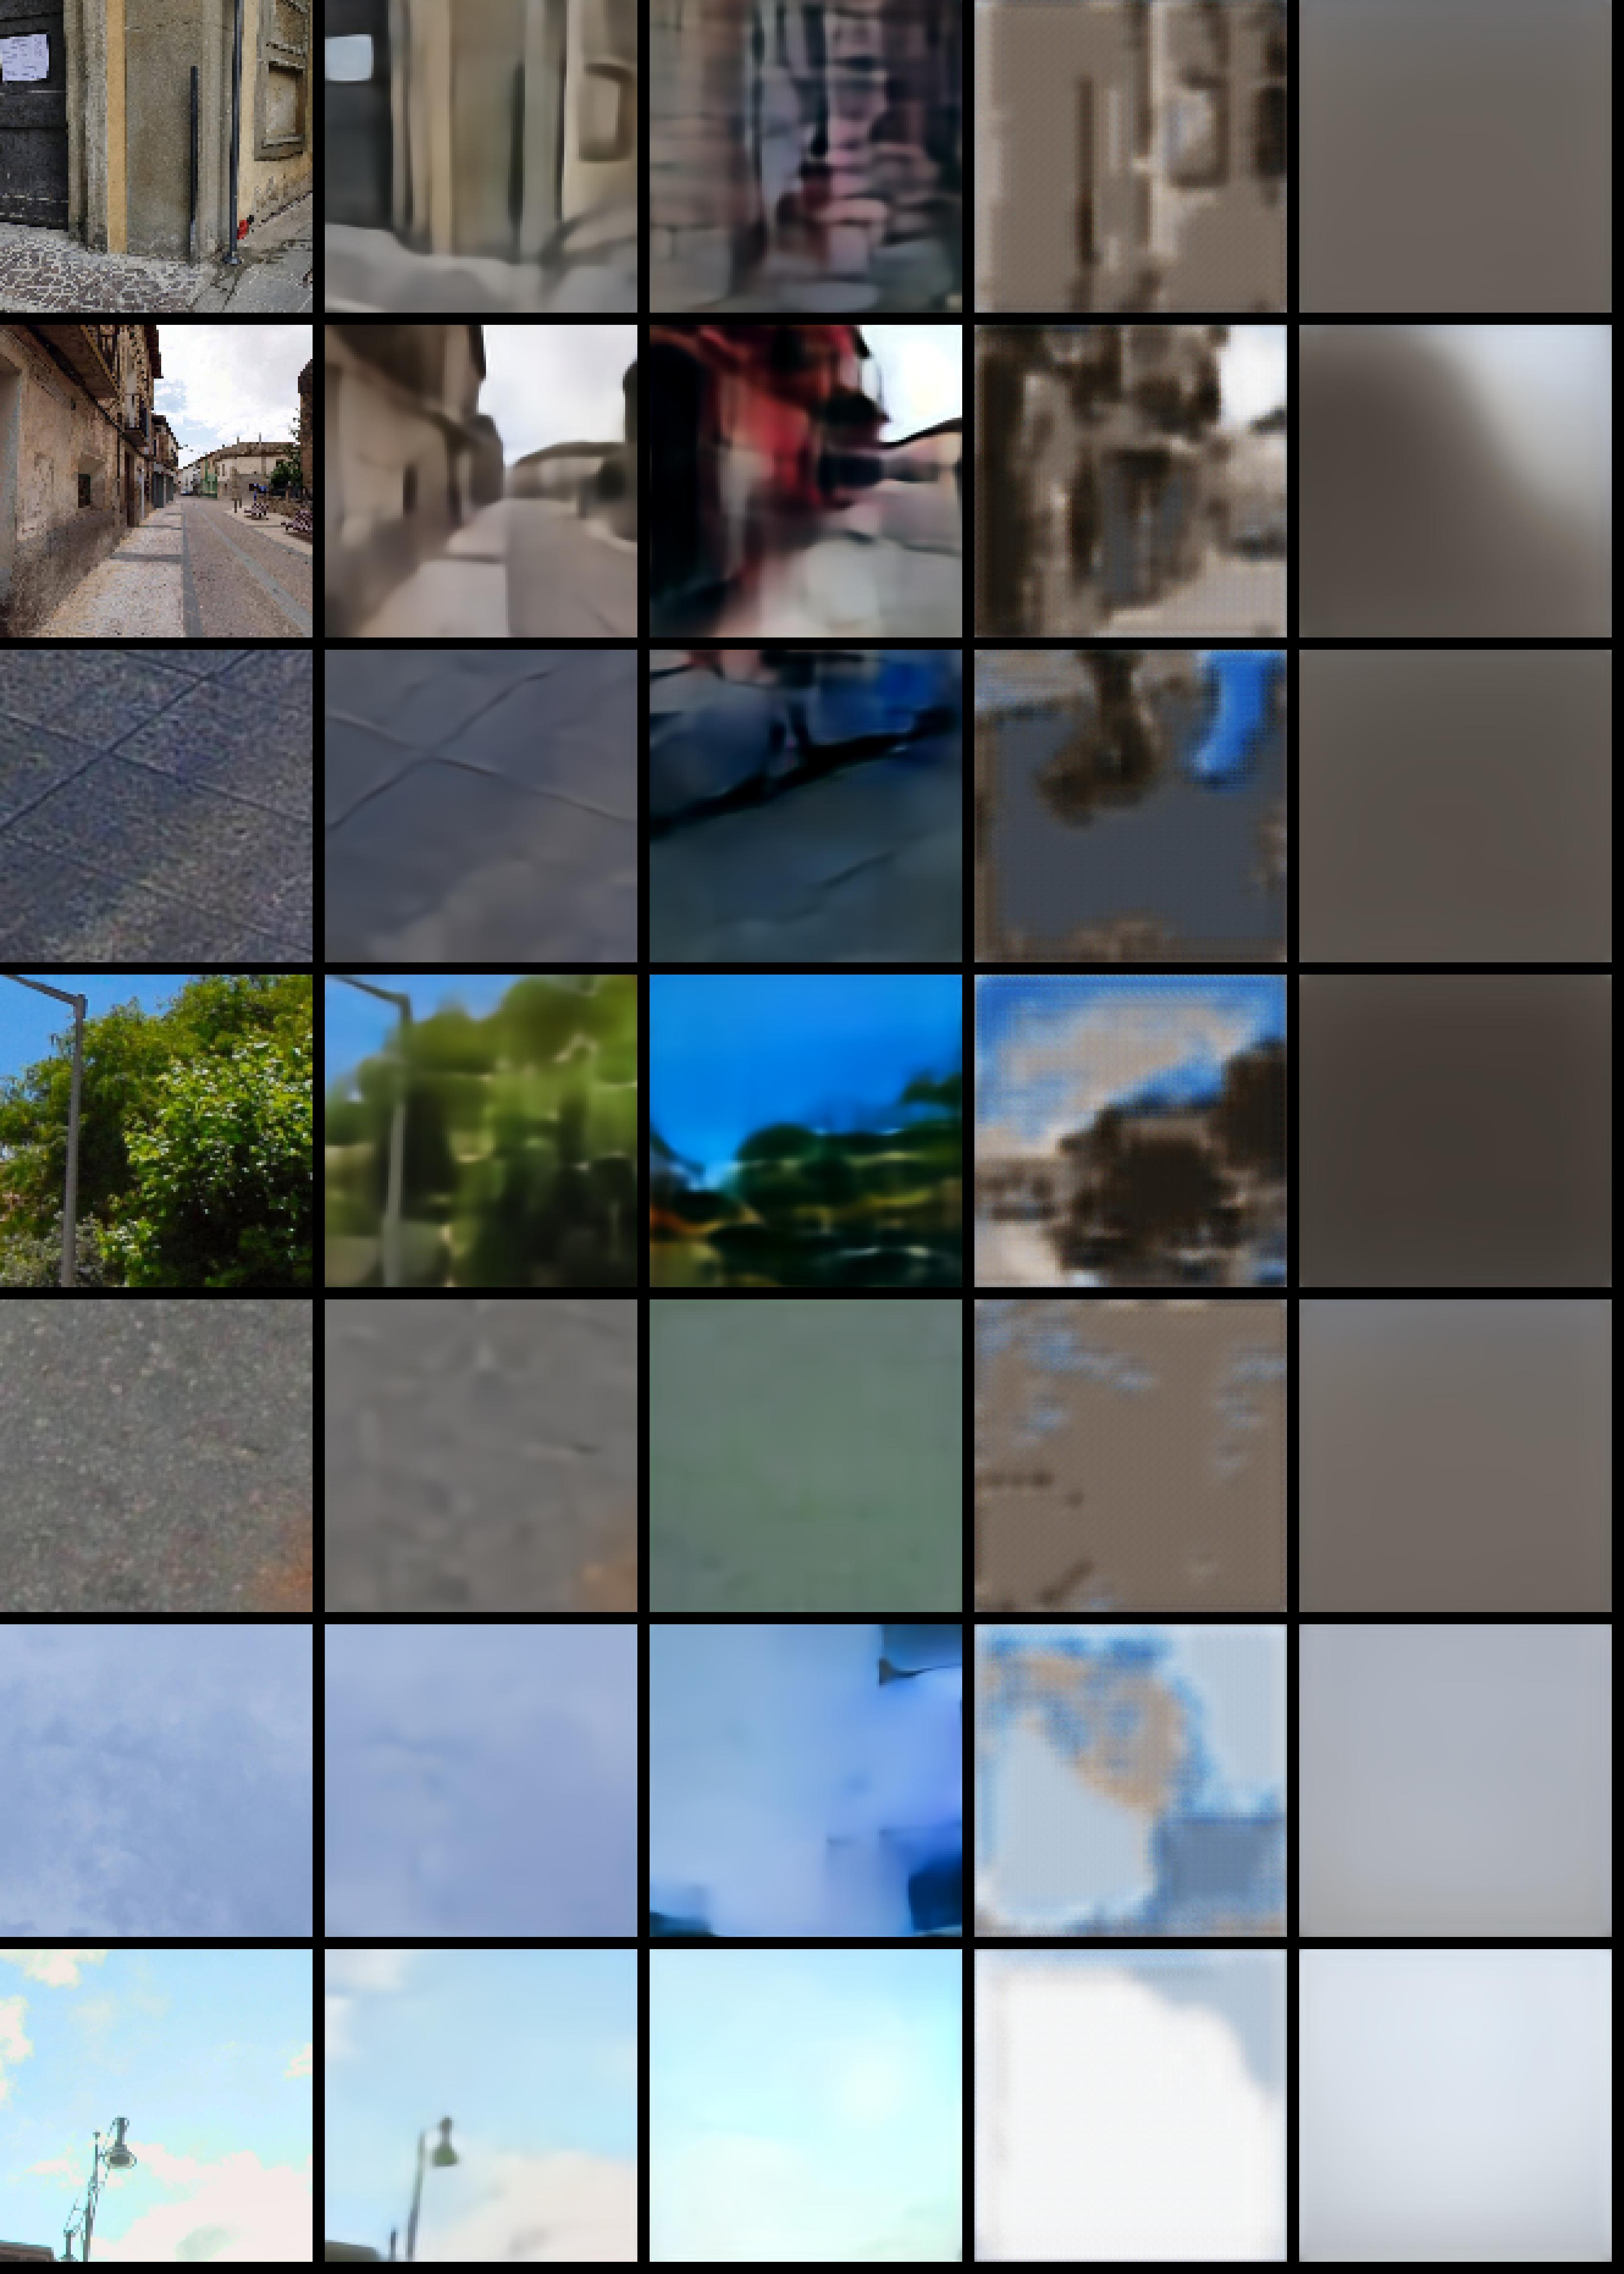
\includegraphics[width=0.85\textwidth]{figures/ptz/test_stacked_1.png}
\end{figure}
\begin{figure}[H]
    \centering
    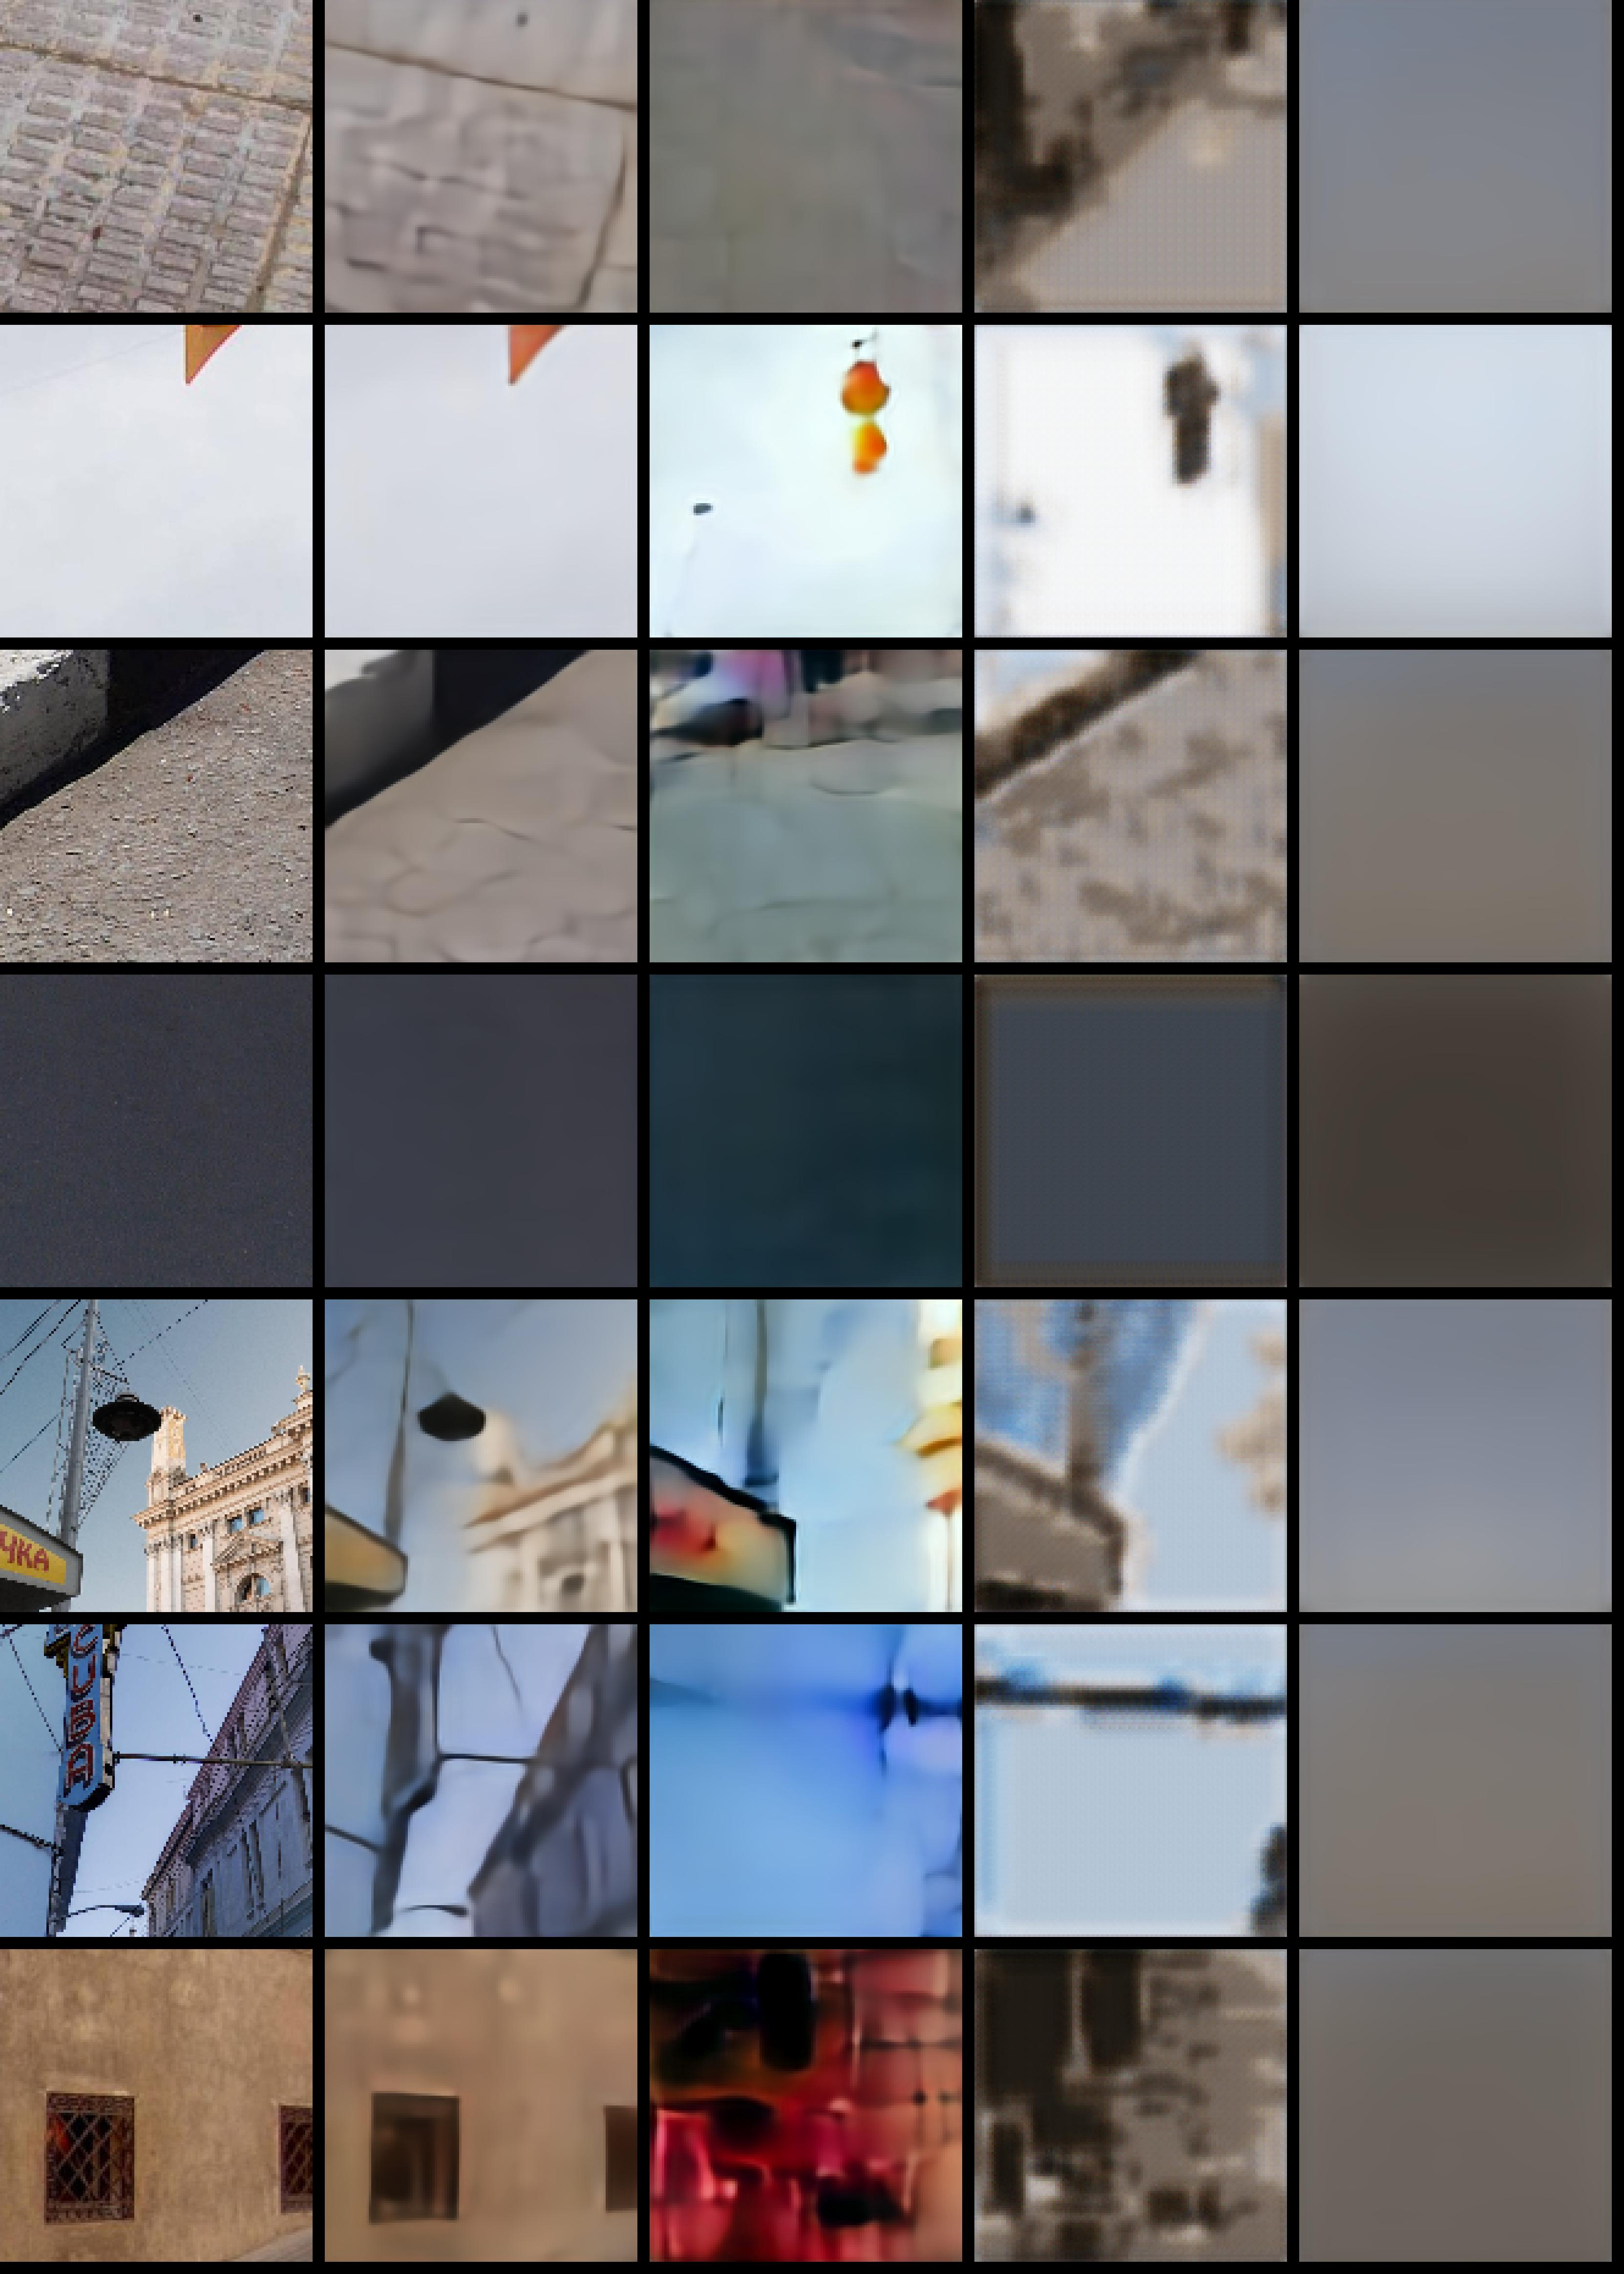
\includegraphics[width=0.85\textwidth]{figures/ptz/test_stacked_2.png}
\end{figure}
\begin{figure}[H]
    \centering
    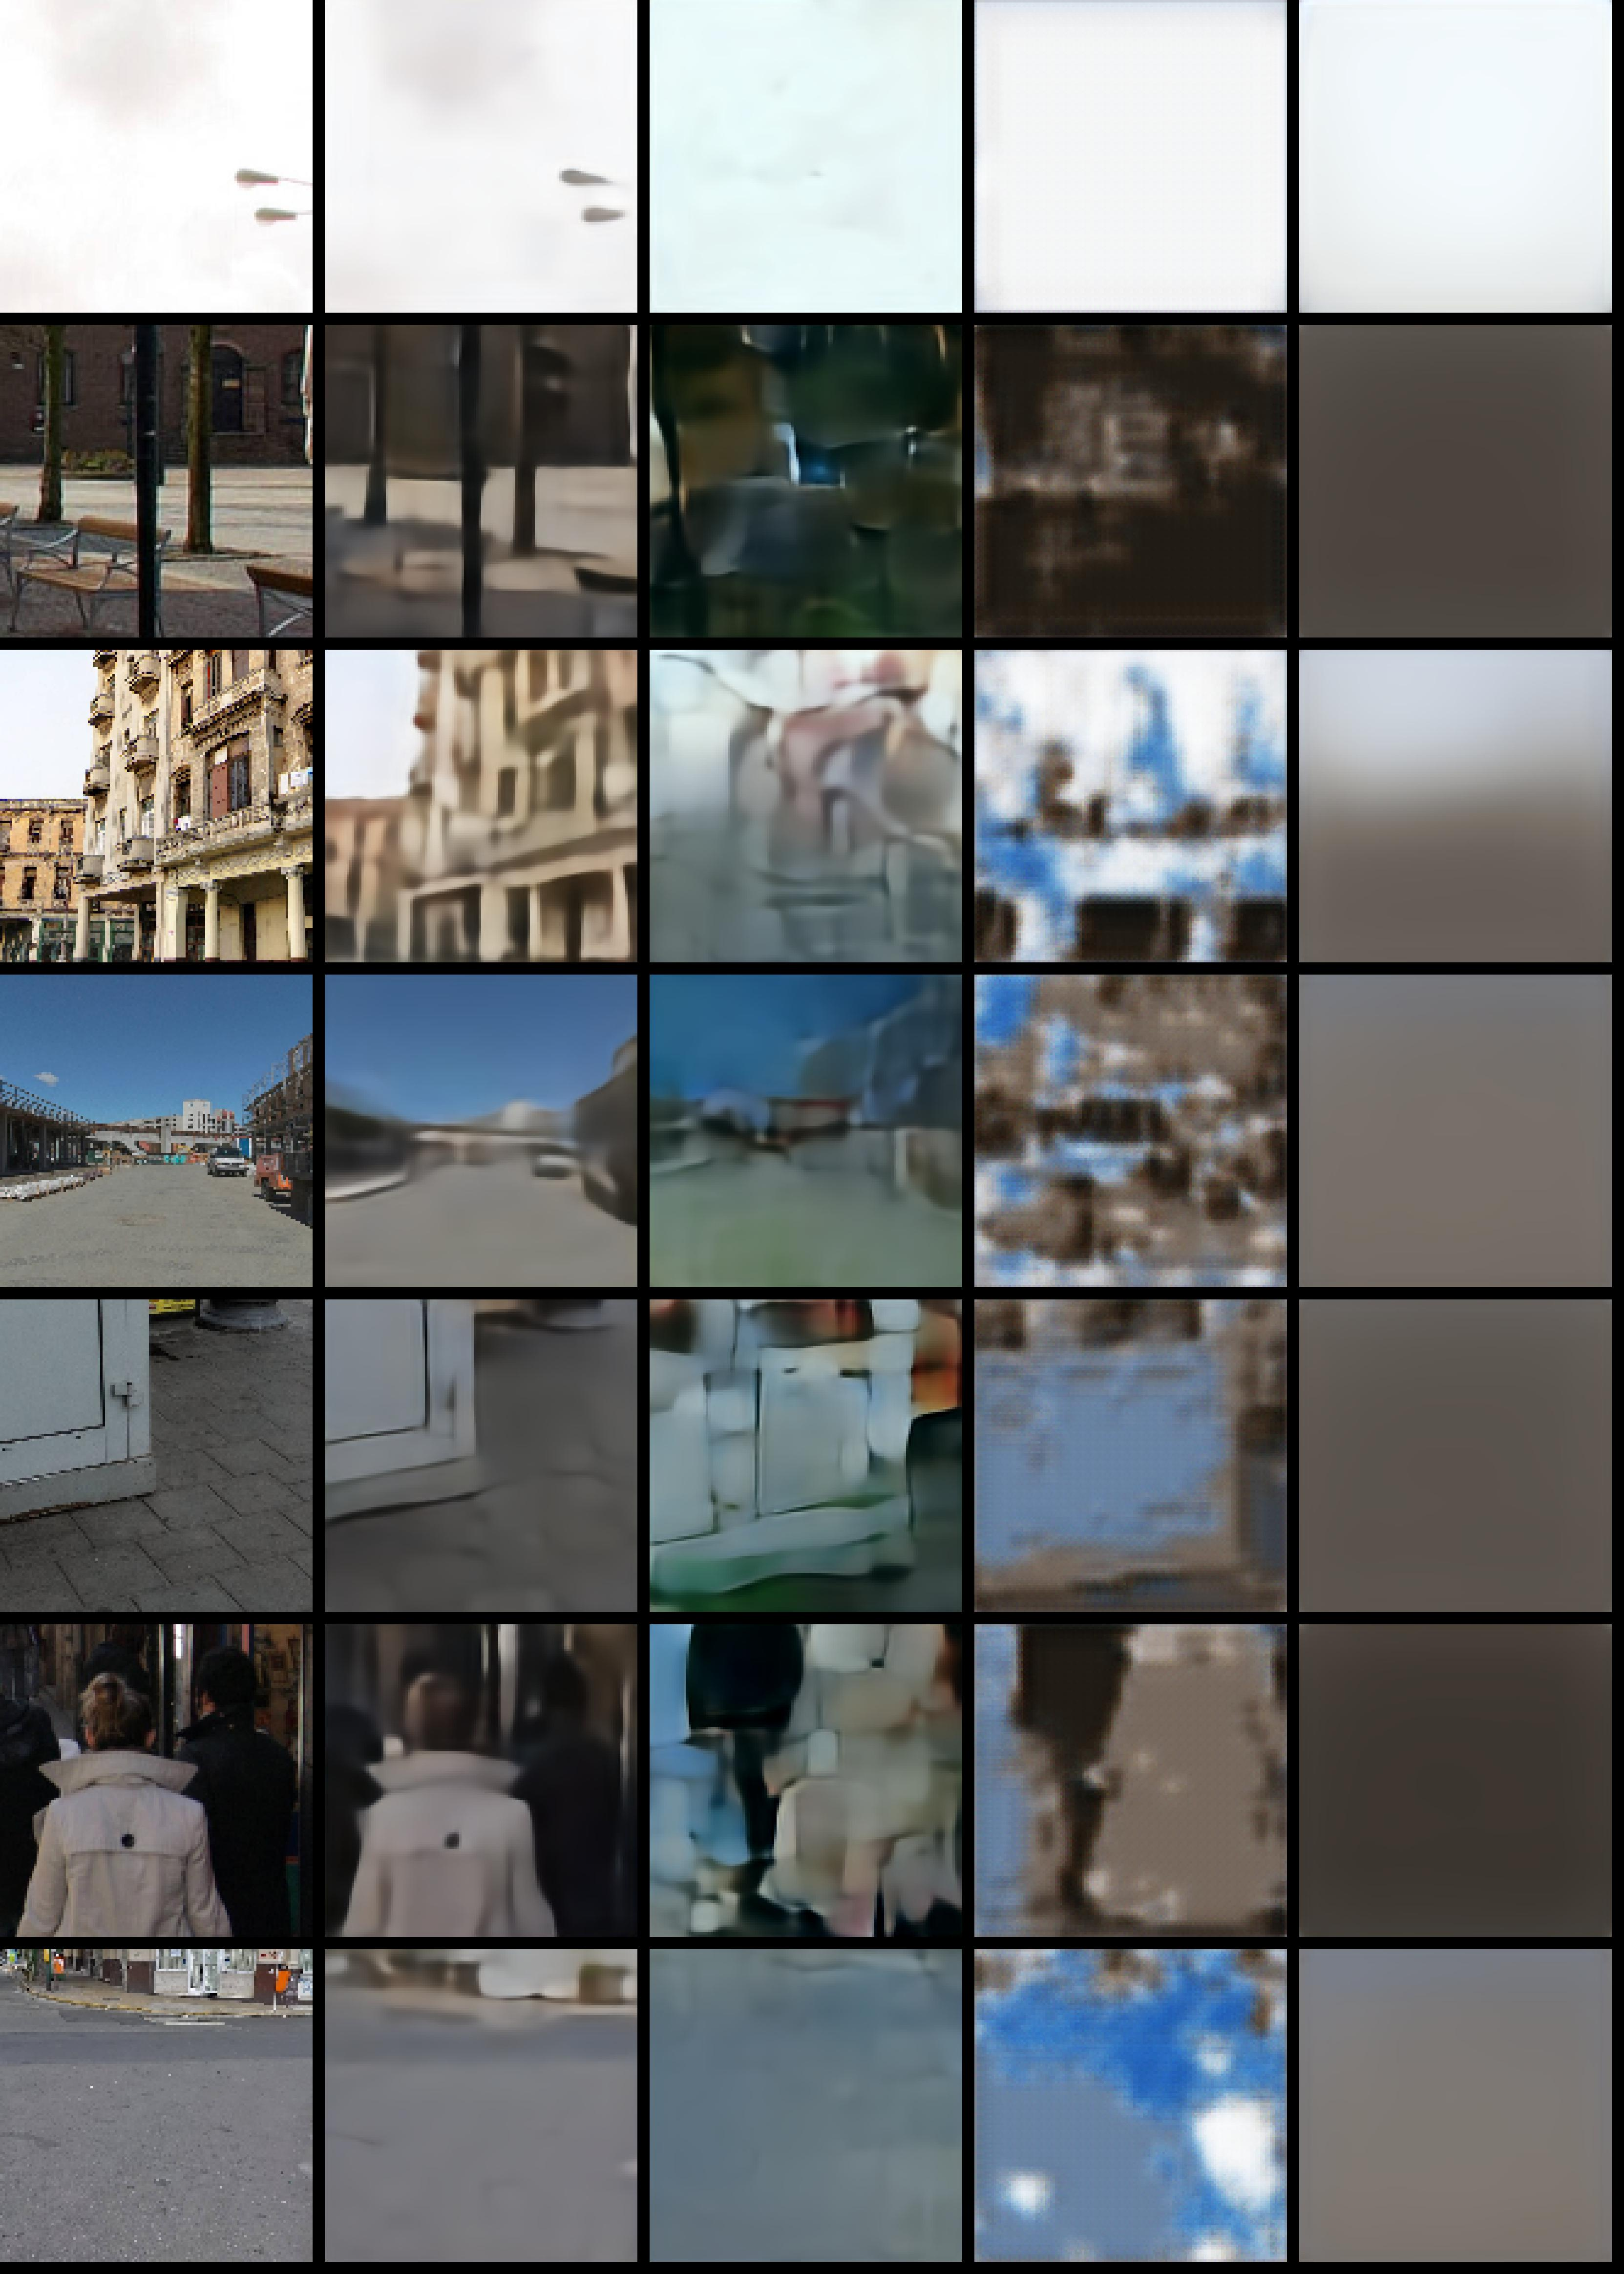
\includegraphics[width=0.85\textwidth]{figures/ptz/test_stacked_3.png}
\end{figure}
\begin{figure}[H]
    \centering
    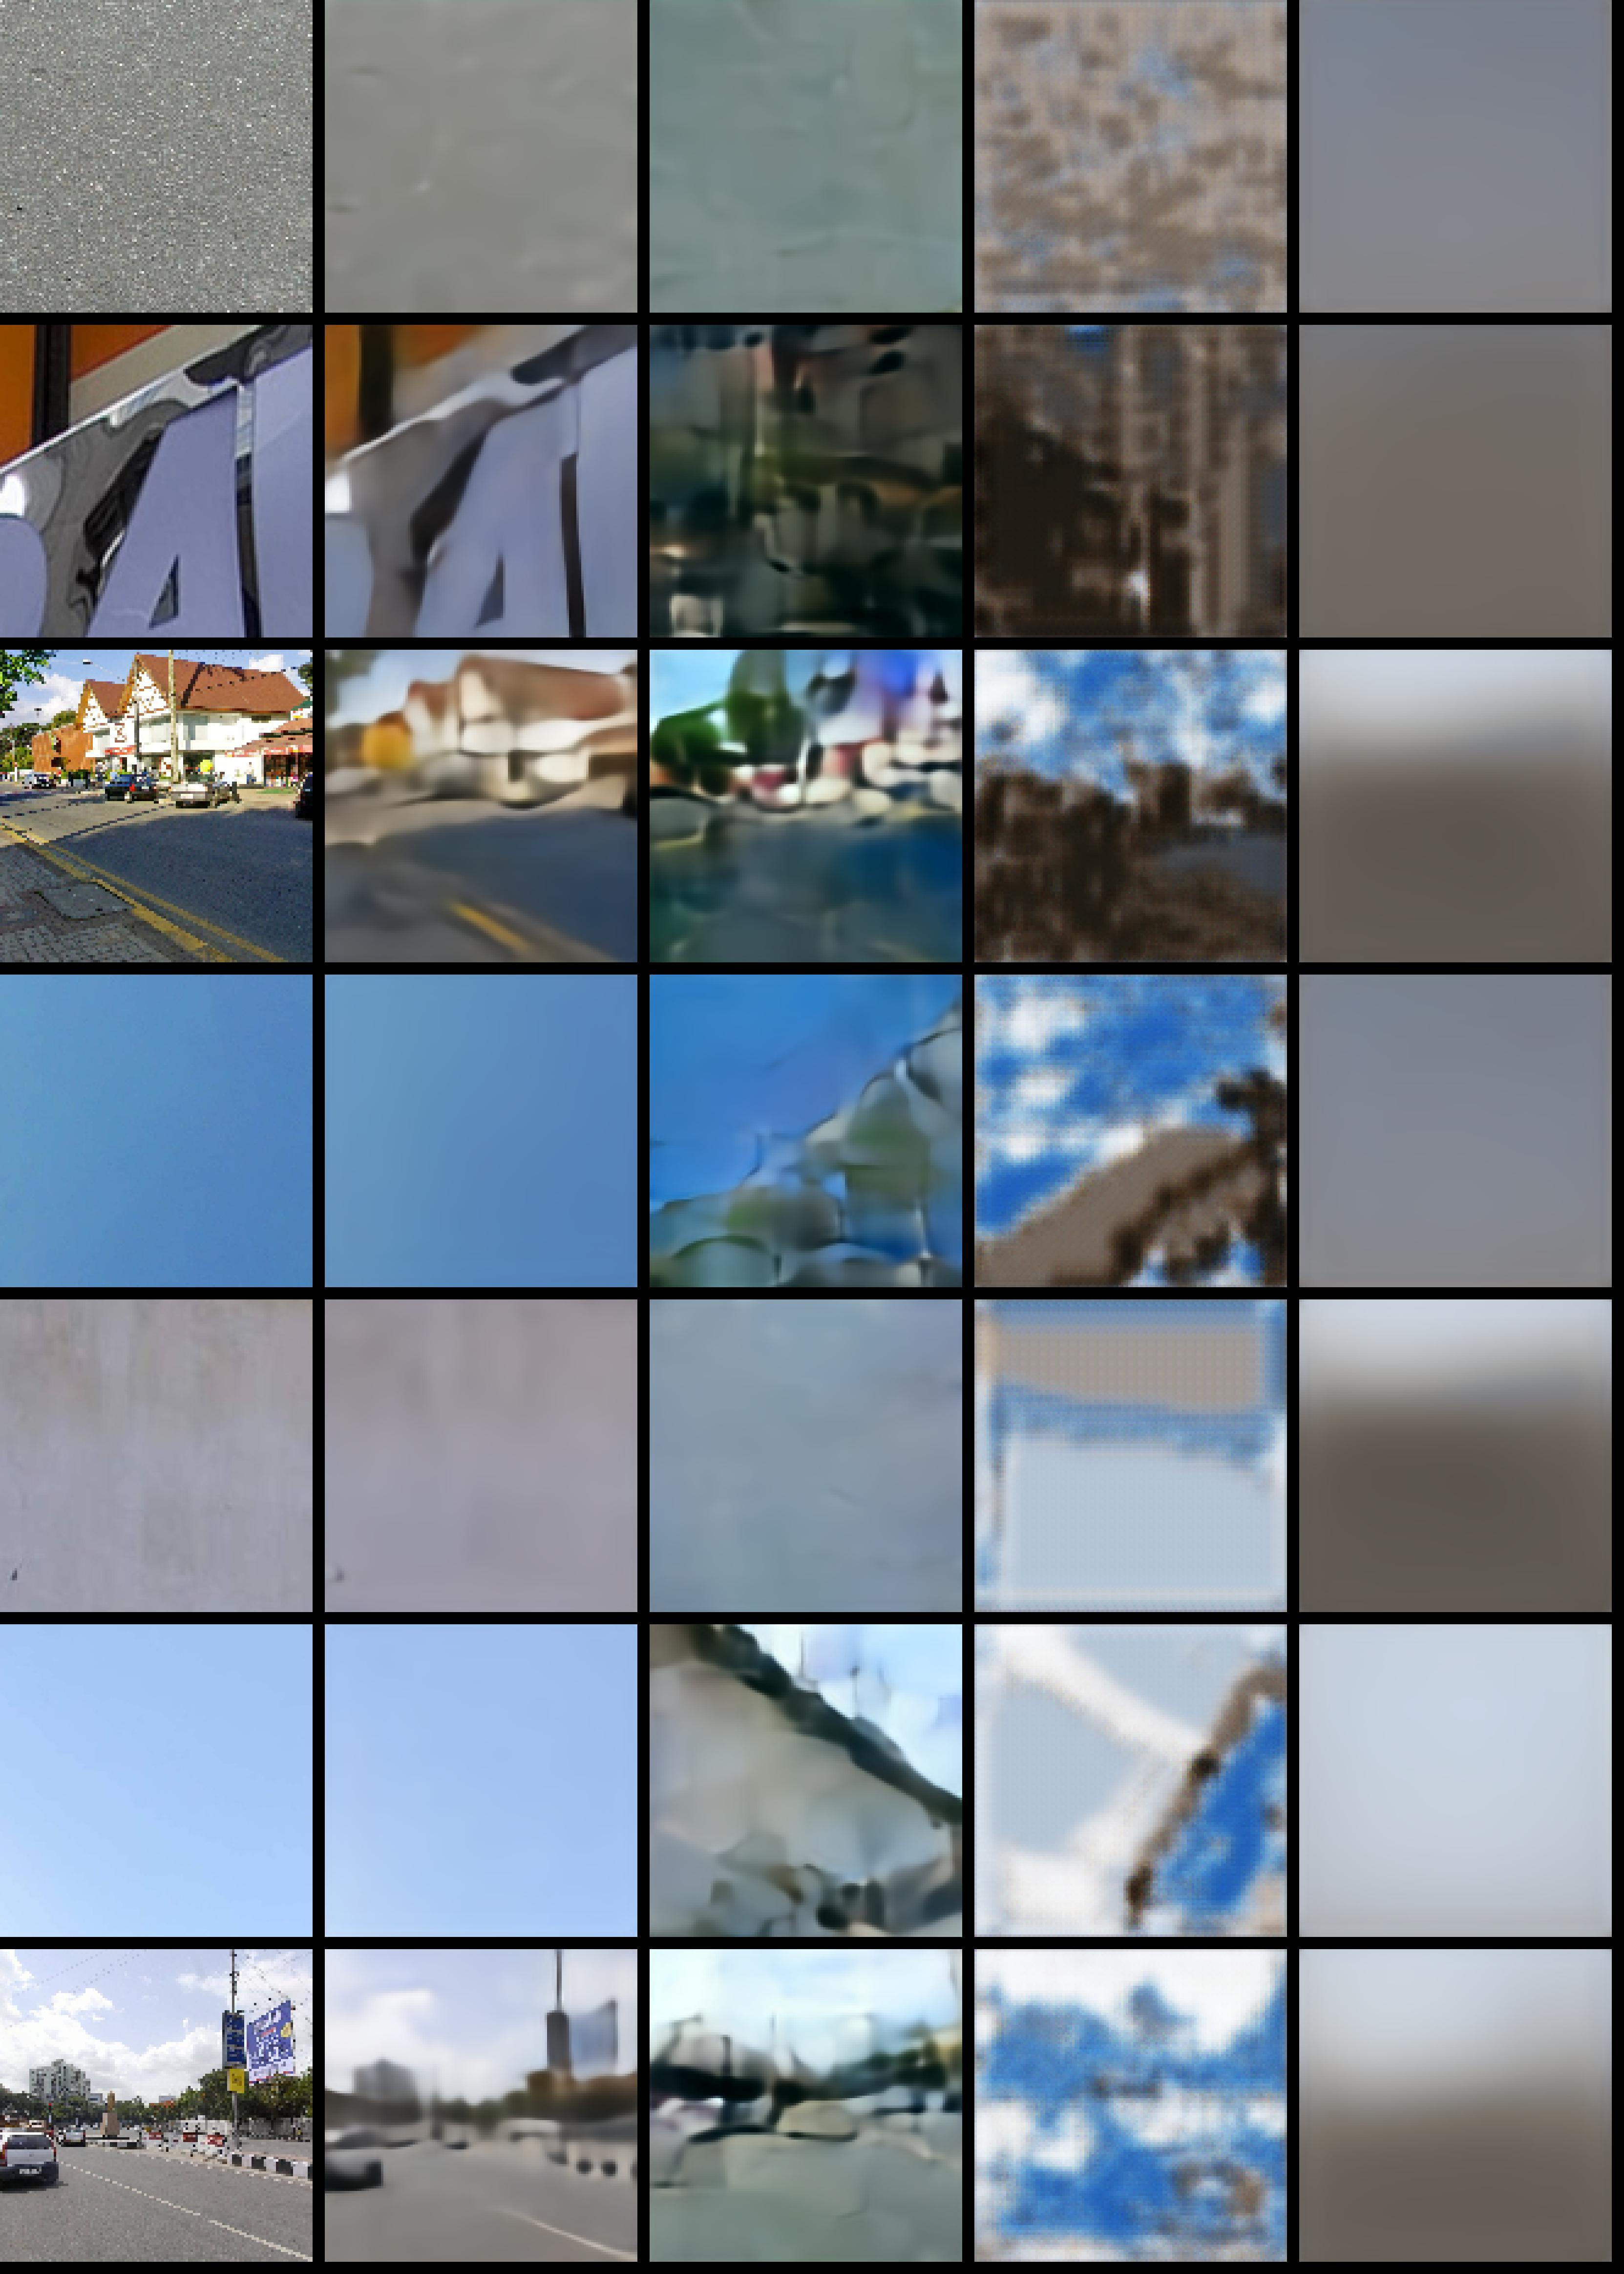
\includegraphics[width=0.85\textwidth]{figures/ptz/test_stacked_4.png}
\end{figure}

\end{appendices}